\documentclass[E5,LUFonts]{lundphdthesis}
% Note using overleaf: Compile with "XeLaTeX" if you want LU fonts

% Possible options:
% E5 or G5 depending on size of thesis book
% LUFonts for using LU chosen fonts
% MathFonts for using the LU chosen fonts for math mode, I don't really think it looks good


% ==================================
% ==================================
% ==================================
%
% FRONTMATTER
%
% ==================================
% ==================================
% ==================================

\title{Stellar kinematics in surveys and simulations}
%\subtitle{subtitle here}   % optional
\author{Daniel Mikkola}

\degree{Thesis for the degree of Doctor of Philosophy}
\titleblurb{Thesis advisor: Dr.\ David Hobbs\\
Co-advisor: Dr.\ Paul McMillan\\
Faculty opponent: Dr.\ Marie Martig}
\announcement{To be presented, with the permission of the Faculty of Science of Lund University, for public criticism in the Lundmark lecture hall (Lundmarksalen) at the Department of Astronomy and Theoretical Physics on the${18}^\textrm{\tiny th}$ November 2022 at 13:00.}

\begin{document}

\maketitleshort   %this one is optional


% ==================================
% "spikningsblad" consists of title with blurb and a data sheet paper
% if the entire spikningsblad is in pdf format these two pages can be handled with includepdf
\maketitlewithblurb
\newpage

% the following overlay the total page number count dynamically, adjust vspace and hspace accordingly
% if too many problems with that, just use \includepdf{datasheet_name} instead
%\includepdf{datasheet_name}
\AddToShipoutPictureBG*{\AtPageLowerLeft{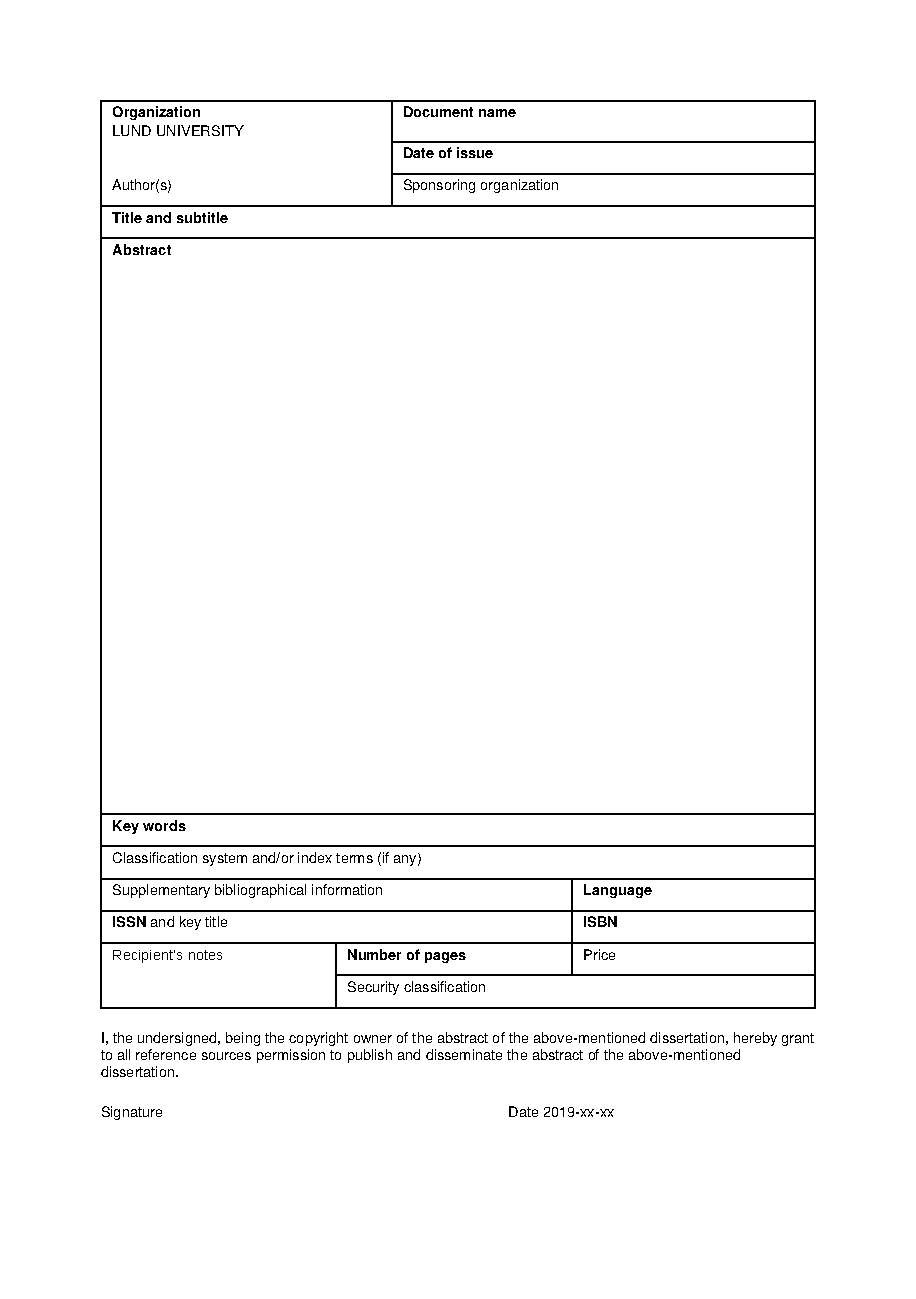
\includegraphics[width=\paperwidth,height=\paperheight]{datasheet_empty.pdf}}}
\vspace*{13.75cm}\hspace*{6.1cm}{\footnotesize\ztotpages}   % modify the distances and font size as needed
\newpage


% ==================================
% actual title page
\maketitle


% ==================================
% make page with evaluation committee and copyright information
\newpage
\begin{center}
	\textbf{Faculty Opponent} \\
	\vspace{1em}
	Prof.\ Someone Someoneson\\
	Department of Astronomy, Someplace University,\\
	Town, Country\\
	\vspace{1.5em}
	\textbf{Evaluation Committee} \\
	\vspace{1em}
    Dr.\ Someone Someoneson\\
    Department of Astronomy, Someplace University,\\
    Town, Country\\
    \vspace{0.7em}
    Dr.\ Someone Someoneson\\
    Department of Astronomy, Someplace University,\\
    Town, Country\\
	\vspace{0.7em}
    Dr.\ Someone Someoneson\\
    Department of Astronomy, Someplace University,\\
    Town, Country\\
\end{center}
\vfill

{\small\parindent0pt
\textbf{Front cover:} Explanation of the front cover.
Credit: xx Edited by xx and printed with permission from xx.

\textbf{Back cover:} .

\textbf{Funding information:} This thesis work is financially supported by -.

\vspace{1em}
\copyright\, Daniel Mikkola 2022

\vspace{1em}
Faculty of Science, Department of Astronomy and Theoretical Physics

\vspace{1em}
ISBN: ~(print)\\ % ISBN av svenska ISBN centralen
ISBN: ~(pdf) % ISBN av svenska ISBN centralen

\vspace{1em}
Printed in Sweden by Media-Tryck, Lund~University, Lund 2022\\

\includegraphics[width=0.5\textwidth]{logo/miljoeloggor}
}

% ==================================
% dedication page
\newpage

\vspace*{140pt}
\begin{flushright}
\textit{Till morfar}
\end{flushright}

% ==================================
% table of contents
\cleardoublepage
\frontmatter
\pagestyle{plain}
\setcounter{page}{1} % Page Roman 1 of the frontmatter
\setcounter{tocdepth}{1}
\setcounter{secnumdepth}{2}
\renewcommand{\thesection}{\arabic{section}}
\tableofcontents


% ==================================
% Work list and popular abstract
\newpage
\sectionhidenum{List of publications}

This thesis is based on the following peer-reviewed publications:
\vspace{1mm}

% \phdarticle{title}{authors}{journal}
\phdarticle{Radial migration and vertical action in N-body simulations}
{\textbf{Mikkola, D.}; McMillan, P. J.; Hobbs, D. (2020)}
{Monthly Notices of the Royal Astronomical Society, Volume 495, Issue 3, pp. 3295-3306}
\phdarticle{The velocity distribution of white dwarfs in Gaia EDR3}
{\textbf{Mikkola, D.}; McMillan, P. J.; Hobbs, D.; Wimarsson, J (2022)}
{Monthly Notices of the Royal Astronomical Society, Volume 512, Issue 4, pp. 6201-6216}
\phdarticle{The velocity distribution of local halo and disk stars in Gaia DR3 from transverse motion}
{\textbf{Mikkola, D.}; McMillan, P. J.; Hobbs, D. (2022)}
{\textit{Submitted to Monthly Notices of the Royal Astronomical Society}}%Monthly Notices of the Royal Astronomical Society, Volume VVV, Issue I, pp. pppp-pppp}
%\phdarticle{Paper 4 title}
%{\textbf{Mikkola, D.}; McMillan, P. J.; Hobbs, D. (2020)}
%{Monthly Notices of the Royal Astronomical Society, Volume VVV, Issue I, pp. pppp-pppp}
%\phdarticle{nishiyama stars ...}
%{\textbf{Thorsbro, B.}; Ryde, N.; Rich, R. M.; ...}
%{In manuscript}
\makephdarticletable


\noindent Papers I, II, and III  are reproduced with permission from Monthly Notices of the Royal Astronomical Society.

\newpage

%\newpage
%\noindent Positions of trust undertaken during the PhD education:
%\begin{enumerate}
%    \item Secretary of the PhD student union at the Faculty of Science, 2017/18.
%    \item Chair of the PhD student union at the Faculty of Science, 2018/19, representing approximately 450 PhD students.
%    \item Chair of the PhD student union at Lund University, 2019/20, representing approximately 2100 PhD students.
%\end{enumerate}

%\vspace{2mm}
%\begin{center}
%\begin{minipage}{0.7\linewidth}
%\textit{``An easily governed university is no university at all.''}
%
%~\hfill\footnotesize{\citep{boultonlucas:08}}  %(Boulton and Lucas, 2008)
%\end{minipage}
%\end{center}


% ==================================
% Popular summary (ENGLISH)
\sectionhidenum{Popular summary}
Of all things on the celestial vault the greatest and most striking is the diffuse band of stars that make up the Milky Way, our home Galaxy. To understand how it formed and evolved we need, among other things, a detailed description of how the stars move and where they are located, the field of research called \textit{astrometry}. The first stellar catalogue was created 200 BCE by Hipparchus in ancient Greece. A little over two millennia later we began measuring stars with space telescopes, the first of which was named \textit{Hipparcos}. This was succeeded by the space telescope \textit{Gaia} which was launched in 2013 and revolutionized the field of astrometry, providing a truly great catalogue of stellar motions and positions. This catalogue has significantly contributed to the research behind this thesis. \textit{Gaia} gives us a very precise picture of how the Milky Way kinematics look today. To complete the picture one also uses numerical simulations to recreate and interpret the features found in observations. The union of theory and observations then reinforce one another and is critical for our understanding of the Milky Way.

The first article in this thesis uses numerical simulations to study how interactions with the Galaxy's spiral arms and bar transports stars radially in the plane of the disc. We find that this migration depends on the Galactic disc's strength and how vertical extended the stellar orbit is. With over 100 simulated discs we could determine that in less massive discs it is mostly the stars close to the disc that migrate and in the opposite case of massive discs they migrate regardless of how far above the disc the orbit goes.

In the second and third articles we use data from \textit{Gaia}. By using positions and velocities along the celestial sphere, without needing velocities in the line-of-sight direction, we have access to extremely large amounts of data. This way, we obtain an estimate for the local stellar velocity distribution, despite lacking one velocity component. We do this for three samples of data. In the second article we used white dwarfs, which are the remains of low mass dead stars, and could discover that there were two separate kinematic populations. In the third article we used the Solar neighbourhood of stars in the disc and a local part of the Galaxy's halo. We were able to identify many known structures in the velocity distribution, as well as some new ones which then belong to the accreted halo, and could be the remains of accreted dwarf galaxies. 


% Utav alla ting på himlavalvet så är det största och mest slående det diffusa band av stjärnor som upppgör Vintergatan, vår hemgalax. För att förstå hur den skapades och utvecklas behöver vi, bland annat, en detaljerad bild av hur stjärnorna rör sig och var det befinner sig. Den första stjärnkatalogen kom 200 f.kr från Hipparchos i antika Grekland. Två millenier senare så började vi mäta stjärnor med rymdteleskop, det första då döpt till just Hipparcos. Detta efterföljdes av rymdteleskopet Gaia, som bidrar stort till forskningen bakom denna avhandling. Detta ger oss en väldigt noggran bild av hur Vintergatans kinematik ser ut idag. För att fullända bilden, använder man sig dessutom utav numeriska simulering som kan återskapa de resultat som vi ser i mätdatan. Föreningen av teori och observationer förstärker då varandra. 

% Den första artikeln i denna avhandling använder just numeriska simuleringar för att titta på hur stjärnor förflyttar sig in och ut från Galaxen på grund av interaktioner med dess spiralarmar och centrala stav. Mer specifikt hur denna migrering beror på Galaxskivans styrka och hur vertikalt utsträckt sjärnans omloppsbana går. Med över 100 simulerade skivor kunde vi bestämma att i gravitationellt svaga skivor migrerar mest stjärnorna nära skivan och i starka skivor migrerar de oavsett vertikal omloppsbana. 

% I den andra och tredje artikeln använde vi mätdatan från Gaia. Genom att vi använder positioner och hastigheter tangentiellt på himlen, utan att kräva hastigheter i siktriktningen, hade vi tillgång till extremt stora mängder data. Vi kan då lokalt få en uppskattning av stjärnornas hastighetsfördelning, även fast vi saknar en hastighet. Detta gjorde vi för tre olika urval av data. I artikel två använde vi vita dvärgar, vilket är kvarlevorna av döda stjärnor, och kunde upptäcka att där fanns två separata kinematiska populationer. I artikel tre använde vi Solens kvarter av stjärnor i skivan och en lokal del av Galaxens halo. Där lyckas vi identifiera många kända strukturer i hastighetsfördelningen, samt några nya som då tillhör den ansamlade halon, och skulle kunna vara kvarlevorna av ansamlade dvärggalaxer. 


% ==================================
% Popular summary (SWEDISH)
\sectionhidenum{Populärvetenskaplig sammanfattning}

%Att utforska världen vi lever i är en del av människans nyfikna natur. Inom astronomi använder vi denna nyfikenhet till att observera universums stjärnor för att försöka förstå hur allt blev till och hur allt hänger samman. I arbetet som presenteras i denna avhandling har vi observerat stjärnor belägna i centrum av vår galax, Vintergatan. Från studier gjorda på andra galaxer vet vi att centrum av en galax hänger samman med hur hela galaxen ser ut och beter sig. Detta samband pekar på att mittpunkten och galaxen som helhet troligtvis utvecklats parallellt.

%Då Vintergatan och dess centrum är den mest närbelägna galaxen vi har, kan vi studera dess egenskaper i stor detalj, jämfört med andra galaxcentra. Om vi antar att Vintergatan är varken mer eller mindre speciell än andra galaxer, kan en god förståelse för Vintergatan och dess centrum lägga grunden för en större förståelse för hur galaxer i allmänhet hänger samman med sina centra.

%I vårt arbete hittar vi både likheter och skillnader mellan stjärnorna som finns i Vintergatans centrum respektive längre ut. Stjärnor består främst av väte och helium men kan även vara berikade med andra grundämnen, beroende på hur och när de har bildats. Både i centrum och längre ut i galaxen hittar vi stjärnor som haltmässigt ser ut att vara lika. Men när det kommer till de mest berikade stjärnorna finns det tydliga skillnader, där centrumstjärnorna har en högre halt kisel jämfört med stjärnor längre ut. Detta kan vara en indikation på att dessa regioner har bildats och utvecklats på olika sätt. Denna kunskap, om man lyckats bekräfta resultaten i framtida studier, är en viktig byggsten i vår förståelse kring Vintergatans utveckling. Som en förlängning kan även denna kunskap användas på andra galaxer och förhoppningsvis ge viktiga ledtrådar till galaxbildning och galaxutveckling i allmänhet.


% ==================================
% Acknowledgements   optional
\sectionhidenum{Acknowledgements}
I am forever grateful to who is probably my greatest supporter, my beloved partner Tina Sörensen who has been by my side ever since I started my doctoral journey. Your unwavering support has been with me through difficult times with debugging, writing, contemplating, and a global pandemic. I would not be where I am today without you. 

My supervisor, David Hobbs. You have mastered the art of knowing when to give a push and when to encourage letting go and taking a step back. You have inspired my work ethic and taken the best care of me as a student of yours. Your door has always been open to me and so has your ear. I will miss walking around the corner to have a chat about just anything.

My co-supervisor, Paul McMillan. Your guidance has been invaluable to me ever since we started working together during my master's project. I am ever impressed by your intuition when looking at new results and to me you have always been a bottomless fount of knowledge. I regret that this is our last project together, however I think I now know what a good enough scientist would do. 

I want to thank the friends I have made at Lund Observatory during my stay here. There are too many master students, fellow PhDs, and staff members I want to thank for me to name them all here. Especially I want to thank Eric Andersson who's thesis has been in tandem with mine, which lead to good friendship over the years. My first and second office-mates Iryna Kushniruk and Bibiana Prinoth, my closest colleagues in almost all matters besides research. You were the ones I could always `turn' to and have a chat about either work of life in general. Wherever I end up in the future I am certain I will not have such a great office situation as the one you have given me. 

I must not forget to thank the Physics \& Lasershow. For almost ten years the show has let me mix work with incredible amounts of fun and given me some of my closest friends. Thank you Per-Olof, Johan Z, Stina, Odd, Johan K, Jonas, Alexandra, Frida, Rebecca, Vassily, Matteus, Lina, David, Elin, and Anna-Maria.  

My friends outside of work: Anton, Sara, Fredrik, Marielle, Rasmus, Anna, Jesper, Lovisa, Johan. You have always made sure to keep me humble and to ask me any and all \textit{astrology}-related questions, much to my bemusement. Adrian, I am thankful we reconnected during our PhDs and could share many hours working out or betraying each other in board games.

To conclude, I want to extent my deepest gratitude to the people who made sure I got here today: my family. First, my parents Marita and Seppo, who always made sure to let me explore while providing all the support I needed. My bonus-mother Suzie, I aspire to have your fortitude. My five brothers Nicholas, Robert, Christopher, Mattias, and Alexander. Of course also my extra family in Halmstad who have always welcomed me. 

%I’m deeply indebted to my lovely wife, Kristina Arnrup Thorsbro, without whom this thesis wouldn't exist. Quitting my well paid job and becoming a student is not a decision you take lightly. Kristina did not so much as flinch at my crazy idea and has been at my side and supporting me every step of the way on this journey.
%
%I would also like to extend my deepest gratitude to my supervisor Nils Ryde, who with his extreme generosity has included me in his scientific collaborations from day one and has trusted me to lead the work on several occasions. Nils Ryde and my co-supervisors, Hampus Nilsson and Henrik Jönsson, have deep know\-ledge of the field, which they have shared willingly and patiently in spite of my constant questioning. For this I am very grateful.
%
%For the writing of my thesis I am deeply indebted to Colin Carlile, Florent Renaud, Rebecca Forsberg and Kasper Brandt Nyegaard; Colin for his meticulous and thorough effort to help me improve my English writing skills, Florent for for being present all summer and willing to discuss all the scientific ideas that I wanted to put in my thesis, Rebecca for helping with such a good translation of my English popular summary into Swedish and Kasper for doing the layout of the front page.
%
%Mike Rich is an inspiration to me with his great enthusiasm for astronomy and extremely wide knowledge of the field. I am especially thankful for our time together at the Keck telescope and being taught how to enjoy life on Hawai'i. I am also very grateful for the time Mike hosted me at UCLA and in his home in Bel Air, Los Angeles---I am looking forward to the next trip.
%
%Mathias Schultheis is also an inspiration to me showing how it is possible to be a great astronomer and still keep both feet grounded on the earth. I am very grateful for the many times that Mathias has hosted me both at the observatory in Nice, but also in his home in Mougins. Who would have thought that it was so productive to sit and work at a beach café at the Côte d'Azur. I am especially thankful for the opportunity to visit and work with Mathias for a month at the observatory in Nice---I can imagine spending more time there!
%
%I am grateful for the collaboration that I have had on the Galactic centre work; in particular Livia Origlia and Tobias Fritz have been along for the entire project and have taught me a lot. A special thanks goes out to Livia for visiting us in Lund and teaching me the ins and outs of the REDSPEC data reduction kit.
%
%The LUMCAS collaboration on laboratory astrophysics with Malmö University has a special place in my time as PhD student. I have greatly enjoyed going almost weekly to Malmö for a fresh change of air, and I am grateful that Per Jönsson, Henrik Hartman, Tomas Brage, Lars Engström and the rest of the crew are so warm and friendly. And yes, let us do that yttrium paper this autumn, it will be great fun!
%
%The Galactic centre project would not have been a reality without the yearly and fantastic work shops in Sexten in the Dolomites, Italy, hosted by Francesca Matteucci and Carlo Morossi. Going there every year, sharing my results and getting incredible feedback has been a corner stone of my work. In particular, discussions at Sexten with Francesca Matteucci and Emanuele Spitoni has provided me with good inspiration.
%
%I am thankful towards Anish Amarsi and Karin Lind for hosting me in Heidelberg, Germany, and teaching me the ways of NLTE calculations. I am also thankful towards Chris Sneden, Greg Mace and Melike Afsar for hosting me at UC Austin, Texas, USA, discussing my work and looking into making future observations with IGRINS a possibility---I hope to get the chance to observe with this instrument.
%
%A special thanks to my friends and colleagues at the Depart of Astronomy and Theoretical Physics. In particular Noemi Schaffer and Eric Andersson for being brilliant office-mates, Lennart Lindegren for being my excellent undergraduate supervisor and Dainis Dravins for sharing his immense depth of knowledge over the years. And a shout out to all the awesome people that have joined for movie nights or a beer at one of the local bars---good times!
%
%Science has not been my only pursuit during my time as a PhD student as I can not help but engage in the organisation I work in, perhaps it is an occupational hazard from being an entrepreneur for more than 15 years. A special thanks goes out to Daniel Michalik for dragging me into student union work, to Andrea Adden for being such a great chair of NDR and teaching me the ropes, to Andrew Lifson, Leif Gellersen and Lea Miko Versbach for taking over after me in NDR. Also a special thanks to Tanya Kolyaka and Liang Zhao for being with me in the LDK presidium, Luis Serratos and Richard Croneberg for their support and Smita Chakraborty and Harsh Shah for having the courage to take over after me. I am very grateful towards all the good and talented people that I have had the opportunity to work with in the student unions. There are indeed many, which gives me hope for the future!
%
%Finally, a special and warm thanks to my family and friends that have always been there for me. It means a lot to me. Jakob Thorsbro, I enjoy your yearly visits to Lund, I always look forward to them.



% Prepare settings for main document
\mainmatter           % Page numbers arabic
\setcounter{table}{0} % Reset table counters to not count the publications table
\setcounter{page}{1}  % Rest page counters, this is where it all starts!

% ==================================
% ==================================
% ==================================
%
% MAIN DOCUMENT
%
% ==================================
% ==================================
% ==================================

\chapter*{Galactic dynamics in the Gaia era}
\addcontentsline{toc}{chapter}{Galactic dynamics in the Gaia era}
\section{Introduction}

%In astrophysics, one of the current and active research topics is understanding the formation and evolution of galaxies \citep{blandhawthorn:16}. Our own galaxy, the Milky Way Galaxy, plays a crucial role, not only because it is the galaxy that we live in, but also because it is the galaxy that we can study in the most detail. Assuming the mediocrity principle, i.e.\ that we are not special, we can use the understanding of our own galaxy to understand galaxies at large.
%
%Our Galaxy is often described as a barred spiral galaxy consisting of number of components, often classified as the halo, the thin and thick disks, the bulge and the Galactic centre \citep{blandhawthorn:16}. Zooming in on the Galactic centre we find that the innermost parts can be described as consisting of a nuclear star cluster hosting a super-massive black hole, with the cluster itself being surrounded by a nuclear stellar disk.
%
%The innermost environment of a galaxy is important for several reasons. Firstly, there are empirical relations between the nuclear star cluster and the entirety of the galaxy it is hosted in. For example we find an empirical relation between the mass of the nuclear star cluster and the mass of the host galaxy. Secondly, almost all galaxies that we observe are found to contain a nuclear star cluster. Thirdly, nuclear star clusters are extremely dense and bright star environments visible from a long way away \citep[see e.g.\ review by][]{neumayer:20}.
%
%In our own Galaxy many of the individual stars of the inner Galactic centre can be resolved and observed separately. Through the technique of spectroscopy the light emitted from these stars can be examined in extreme detail giving us insight into information about the stars, most notably the chemical composition of the stars \citep[see e.g.][]{spectrophysics:1999,stellaratmospheres:2014}.
%
%All chemical species beyond the very lightest species are formed by various different fusion processes in the stars, or in some cases during the merger processes of stars \citep{kobayashi:20}. Thus, the observation of different chemical species are a consequence of, and hence a witness to, the existence of these fusion processes. Which fusion process happens is dependent on several factors, most notably the mass of the star and whether or not the star is part of a binary star system, described in more detail in stellar evolution theories \citep[see e.g.][]{prialnik:00}. Chaining together the lives of many stars accumulates a production of chemical species that eventually combines into a mixture of chemical species that we can observe today. The chemical species mixtures are thus fingerprints of the history of the given environments the mixtures are observed in.
%
%In other words, by observing the chemical composition of stars, we are able to set constraints on, or provide clues to, how the environments that stars reside in, have formed and evolved.
%
%In Section~\ref{sect:galaxyevolution} galaxy formation and evolution theories and how they relate to the work in this thesis are described briefly and in Section~\ref{sect:chemicalevolution} an overview of basic chemical evolution is given. Following in Section~\ref{sect:observations} is an account of the observations that have provided the data. Finally, in Section~\ref{sect:spectroscopy} the methodology of spectroscopy, which is the foundation of the work done in this thesis, is described in more detail. In the second part of this thesis the author's contributions to the scientific articles are described and the articles themselves are included.
\addcontentsline{toc}{section}{Paper I}
\addcontentsline{toc}{subsection}{Galactic kinematics}
\section{Galactic kinematics}\label{sect:galactickinematics}

%Firstly an introduction to galaxies is given, and afterwards galactic formation and evolution models are considered. This is followed with a discussion on how the theories form predictions that call for observations to constrain the theories.
%
%\subsection{Galaxies}
%
%Galaxies have been called the building blocks of the Universe and are in general seen as the home of stars. Knowing a few basic facts about galaxies, and in particular our own galaxy, the Milky Way, is beneficial to getting an idea of the overarching astronomical context of the work discussed in this thesis.
%
%A galaxy typically has a radius of the order of several kpc and a mass, not including dark matter, between $10^{7}$\,M$_\odot$ and $10^{12}$\,M$_\odot$ and is self gravitating. The Milky Way galaxy is estimated to have a radius of about $25\pm10$\,kpc with the Sun located about 8\,kpc from the centre and has a mass of stars and other baryonic material of about $6 \cdot 10^{10}$\,M$_\odot$. Extending the radius out to about 200\,kpc and including the dark matter halo the mass of the Milky Way reaches upwards to $10^{12}$\,M$_\odot$ \citep{blandhawthorn:16}.
%
%Galaxies come in various forms and shapes and the two dominant classifications are spherical and spiral galaxies, often called respectively early type and late type galaxies. The classifications can further be subdivided, for example a spiral galaxy can have a bar or not, and there can be several disk components. The Milky Way is considered to be be a barred spiral galaxy with a bulge and both a thin and thick disk surrounded by a halo, as illustrated in Figure~\ref{fig:milkywaysketch}.
%\begin{figure}[t]
%    \centering
%    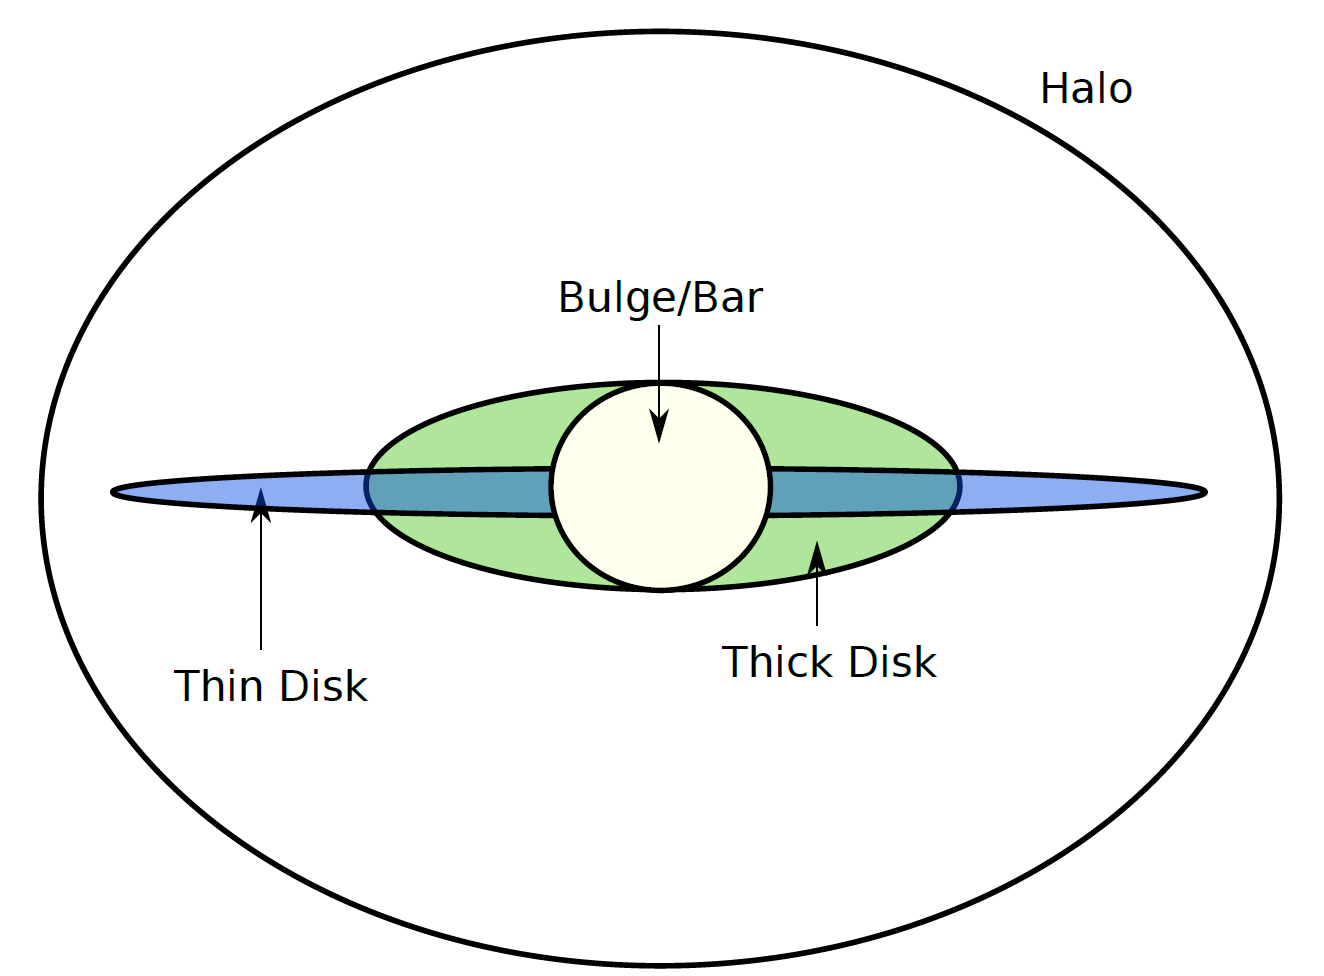
\includegraphics[width=0.8\textwidth]{images/milkywaysketch.png}
%    \caption{A schematic illustration of the stellar components of the Milky Way. The thick disk is illustrated in green, the thin disk in blue and the bulge/bar in beige. The stellar halo surrounding it all is in white. Adapted from \citet{ivalubarlachchristensen:master} with permission.} % Fig. 1.1
%    \label{fig:milkywaysketch}
%\end{figure}
%The bulge is thought to have a mass of about $1.8 \cdot 10^{10}$\,M$_\odot$, the thin disk about $3.5 \cdot 10^{10}$\,M$_\odot$, the thick disk about $6 \cdot 10^9$\,M$_\odot$ and the stellar halo about $4$-$7 \cdot 10^8$\,M$_\odot$ \citep{blandhawthorn:16}.
%
%Almost all galaxies we observe have a bright stellar nucleus, a so-called nuclear star cluster, at their centre \citep{neumayer:20}. The Milky Way is no exception, and has a nuclear star cluster with a radius of about 5\,pc having a mass of about $2.5 \cdot 10^7$\,M$_\odot$. Surrounding the nuclear star cluster is a nuclear stellar disk that extends out towards $150$-$200$\,pc radius and has a mass of about $1.5 \cdot 10^9$\,M$_\odot$ \citep{blandhawthorn:16}. Note, that the distances are now of the orders of pc instead of kpc, which serves to illustrate that these regions have a very high density of stars. At the centre of the nuclear star cluster in the Milky Way lies a supermassive black hole with the mass of about $4.2 \cdot 10^6$\,M$_\odot$ \citep{blandhawthorn:16}. Supermassive black holes have been detected in many galaxies, but are not as ubiquitous as nuclear star clusters \citep{neumayer:20}.
%
%Nuclear star clusters have been found to have empirical relations with their host galaxy, suggesting that nuclear star clusters may have coevolved with their host. Studying nuclear star clusters thus potentially becomes key in understanding the galaxies they are located in, which is particularly interesting as nuclear star clusters are very dense star environments making them bright targets that can be observed from much further away compared to other parts of their host galaxy. One particularly interesting relationship is that between the mass of the nuclear star cluster and the mass of its host. The mass relationship is shown in Figure~\ref{fig:nscrelation}.
%
%\begin{figure}[t]
%    \centering
%    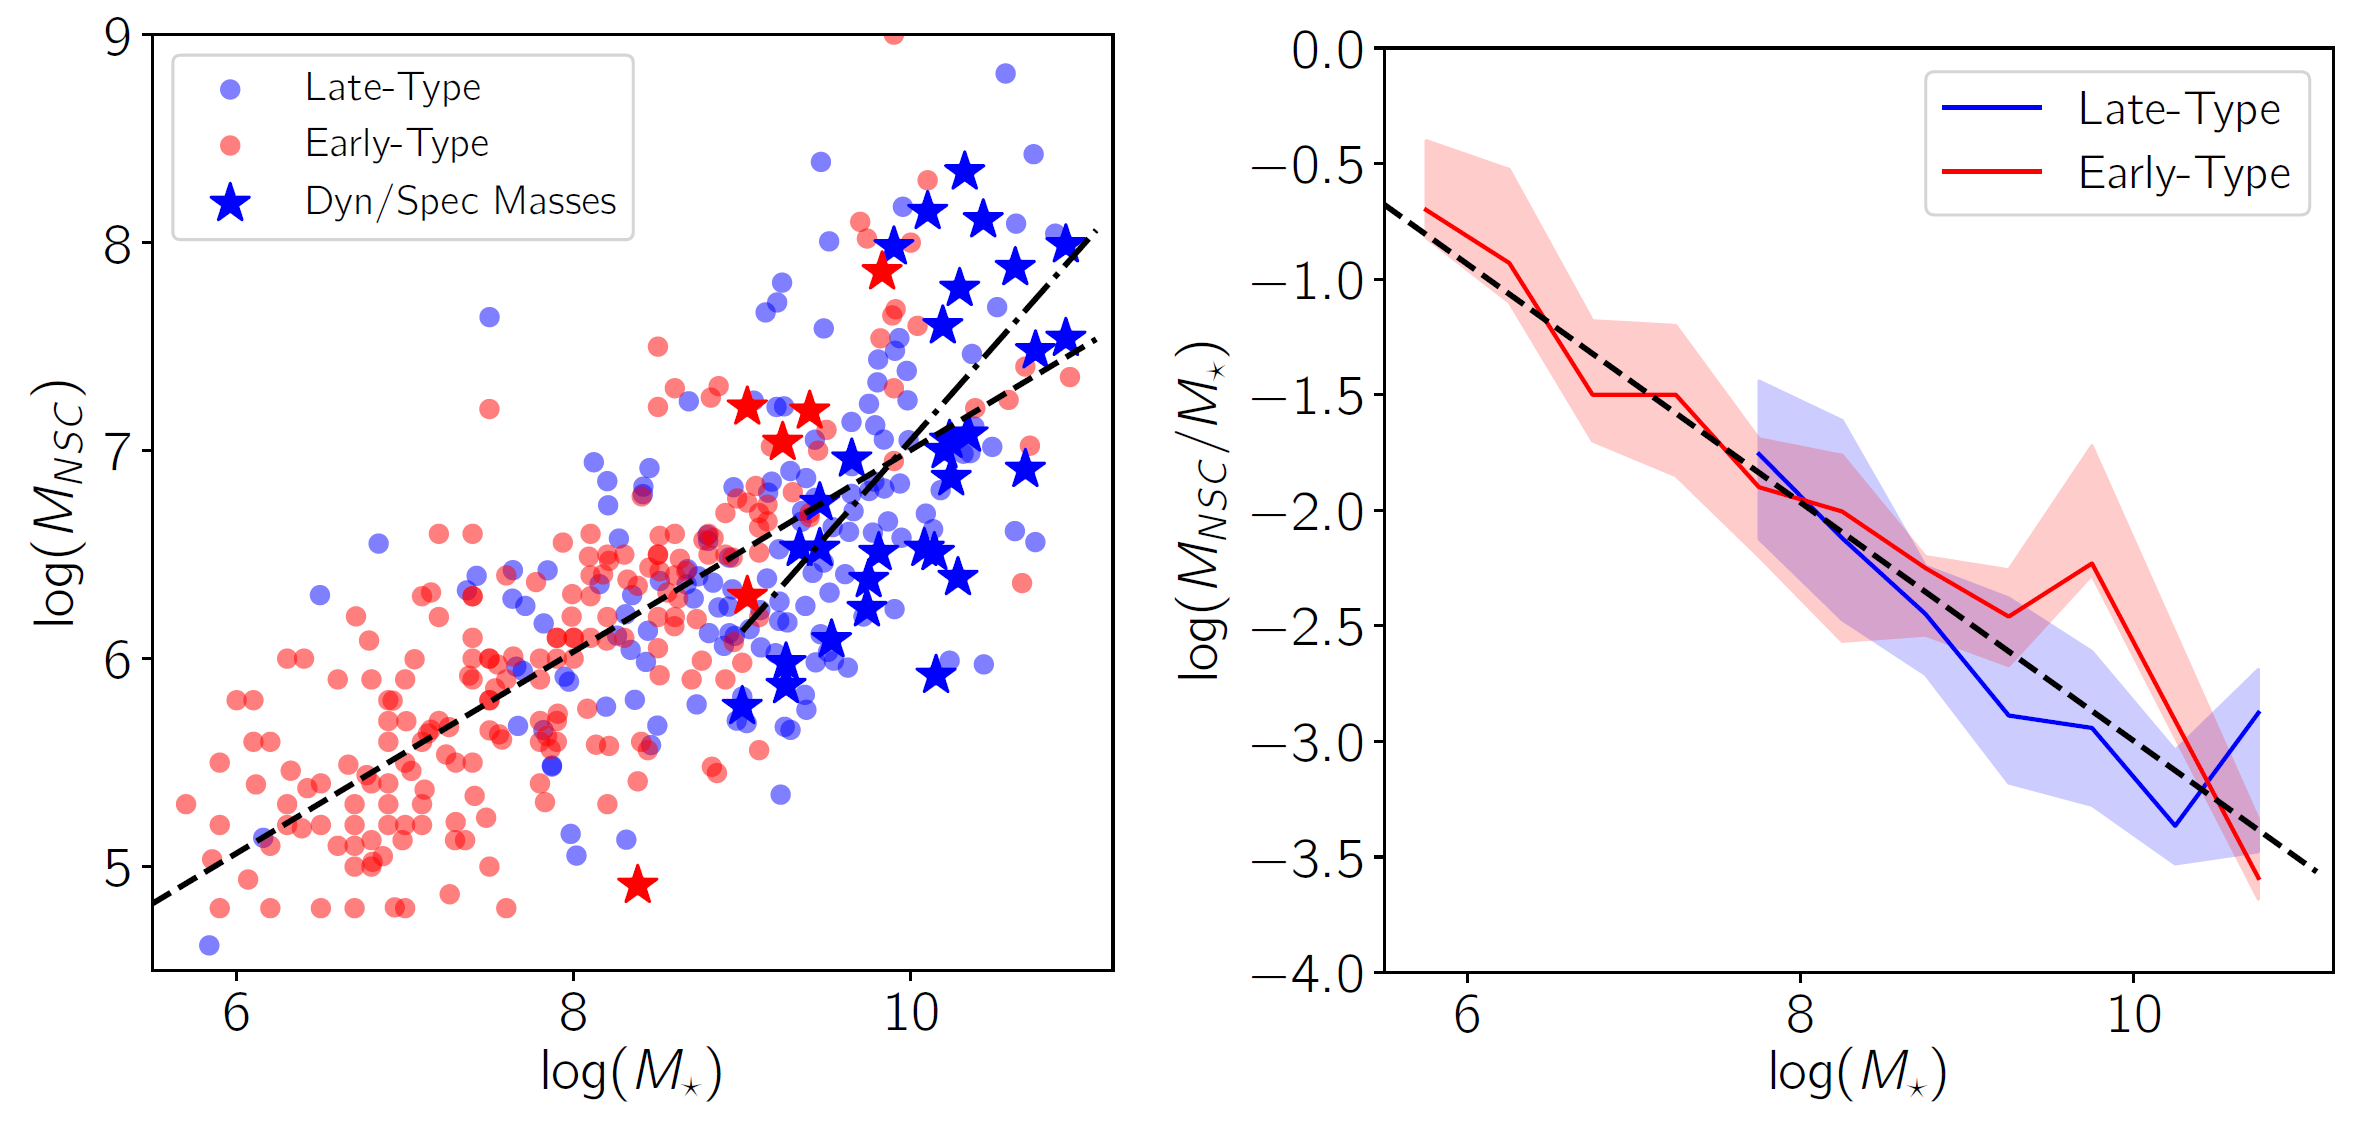
\includegraphics[width=1.0\textwidth]{images/nscrelation}
%    \caption{The masses of nuclear star clusters (NSCs) correlate with galaxy masses, but higher-mass galaxies have a lower fraction of their mass in their NSC. \emph{Left} -- NSC mass vs.\ Galaxy mass ($M_\star$). The disks and stars represent different methods of determining the masses of the NSCs, see the text for more information. The full sample is fitted to the dashed line, while the dashed-dotted line is a fit to the subset marked with blue stars. Galaxies have been divided by their Hubble types into early (red) and late (blue) types. \emph{Right}~-- The mass fraction of galaxies in NSCs as a function of galaxy mass, using the data from the left panel. The line indicates the median galaxy within each mass bin, while shaded regions show the 25th and 75th percentiles of the distribution. Adapted from \citet{neumayer:20} with permission.} % Fig. 12
%    \label{fig:nscrelation}
%\end{figure}
%
%In Figure~\ref{fig:nscrelation} in the left pane, the masses of the nuclear star clusters are shown in relation to the masses of their host galaxies. The disks and stars represent two different studies. The star symbols refer to a study done by \citet{erwin:12b} where the mass of the studied nuclear star clusters either have been dynamically measured or obtained by fitting multiple single stellar populations to high resolution spectra. The disks represent studies where multiple single stellar populations have been fitted to colours obtained through photometry \citep{georgiev:16,spengler:17,ordenesbriceno:18,sanchezjanssen:19}. %The concept of single stellar population will be described in more detail in the next section below on formation and evolution.
%
%Fitting the total sample to a linear relationship gives the dashed line seen in Figure~\ref{fig:nscrelation}, given by \citet{neumayer:20} as
%\begin{equation}
%    \log M_\textrm{NSC} = 0.48 \log \left( \frac{M_\textrm{host}}{10^9 \textrm{M}_\odot} \right) + 6.51.
%\end{equation}
%More simply put the mass of nuclear star clusters are proportional to the square root of the mass of their host galaxy. If one considers the methods used by \citet{erwin:12b} to be more accurate and precise then there more uncertain photometric based methods used by the other authors, and focus on late-type galaxies (i.e.\ spiral galaxies like the Milky Way) the relationship looks rather different, which is marked by the dashed-dotted line in Figure~\ref{fig:nscrelation}, given by \citet{neumayer:20} as
%\begin{equation}
%    \log M_\textrm{NSC} = 0.92 \log \left( \frac{M_\textrm{host}}{10^9 \textrm{M}_\odot} \right) + 6.13.
%\end{equation}
%Here the relation between the mass of the nuclear star clusters and their host galaxies is almost linear.
%
%Examining these relationships using the Milky Way data shows good agreement with either of the relations. They both adequately describe the relation between the mass of the Milky Way nuclear star cluster, $2.5 \cdot 10^7$\,M$_\odot$, and the mass of the Milky Way itself, $6 \cdot 10^{10}$\,M$_\odot$. In Figure~\ref{fig:nscrelation}, the Milky Way would be plotted near the intersection of the two lines.
%
%With an overview of galaxies in place, from a viewpoint that focuses on their centres, we turn our attention to their formation and evolution.
%
%\subsection{Formation and evolution of galaxies}
%
%Theories of formation and evolution of galaxies should be able to explain the galaxies we observe today, particularly the Milky Way, where observations provide much greater detail.
%
%With the advent of strong computational power in the last two decades, numerical simulations using first principles of fundamental physical laws combined with appropriate physical modelling have become one of the dominant methods for investigating galaxy formation and evolution \citep[see e.g.\ review by][]{naab:17}.
%
%The starting point for any theory of formation and evolution is the initial conditions. Modern cosmological models describe the Universe after the Big Bang and also how the structure of the Universe was initially formed. The initial baryonic matter in the Universe is described as a primordial gas consisting of hydrogen and helium, with helium having a mass fraction of about 24\% \citep{extragalacticbook}. The density of the primordial gas is not perfectly uniform initially, leading to the over-density regions amplifying with gravity over time to form the large scale structures, and finally the galaxies \citep[e.g.][]{mo:98}.
%
%In simulations based on cosmological models a Milky Way--like galaxy is typically formed by mergers of smaller galaxy fragments early on. Examples of such simulations are the EAGLE simulation \citep{eagle:i,eagle:ii}, the AURIGA simulation \citep{auriga:i} and the recent VINTERGATAN simulation \citep{vintergatan:i,vintergatan:ii,vintergatan:iii}.
%
%The limiting factor for simulations is computational power, and thus the different simulations vary in both the volume of space they cover and the shortest distances they can resolve in their simulated space. Furthermore, the simulations can be run multiple times to explore different initial conditions and increase statistics. The EAGLE simulation covers a very large volume of space, enough to contain about 10,000 Milky Way--mass galaxies, but has poor resolution ($\sim1$\,kpc). The AURIGA simulation focuses on simulating a single Milky Way--like galaxy, with intermediate resolution ($\sim200$\,pc), and runs the simulation 30 times with varying initial conditions to build up statistics. The VINTERGATAN simulation also focuses on simulating one Milky Way--like galaxy, having only one instance, but at very high resolution ($\sim20$\,pc).
%
%Alternatively, one can start with one large gas cloud and form a galaxy from that without accounting for the cosmological context, as a means of studying an isolated galaxy, which arguably the Milky Way could be. A recent example of such a simulation with multiple realisations has been done by \citet{khoperskov:20}, having a high resolution ($\sim50$\,pc).
%
%A major goal of the simulations mentioned above is to show how galaxies with a Milky Way--like morphology can be formed. While this is undoubtedly an important diagnostic, there are also other diagnostics available to us. One such diagnostic is the chemical composition of the atmospheres of the stars found in various parts of a galaxy. The underlying theories for this diagnostic are covered in more depth in Section~\ref{sect:chemicalevolution} on chemical evolution models. Common to the simulations mentioned above is that they all include this diagnostic, i.e.\ provide the chemical composition of the atmospheres of the stars found in the simulations.
%
%The chemical compositions of the atmospheres of stars can be observed in the Milky Way and its satellite dwarf galaxies where it is possible to resolve individual stars and determine their chemical composition using spectroscopy. It is not possible to resolve individual stars in other galaxies than these. However, with the advent of 30-40 meter telescopes now in construction, resolving stars in the neighbouring Andromeda galaxy, M31, should become possible \citep[see proposals by e.g.][]{escala:20}. This diagnostic is an example of how the greater detail of the Milky Way available to us enhances the demands on the theories.
%
%When discussing the chemical composition of the atmosphere of stars, one of the most commonly used approaches is to examine the ratio of alpha-abundance to iron-abundance of a star vs.\ the metallicity of the same star. The alpha-elements are the stable atoms with a nucleus comprised of a certain number of alpha-particles (2 neutrons and 2 protons), which are C, O, Ne, Mg, Si, S, Ar and Ca. The metallicity of stars is usually measured through the proxy of the ratio of iron to hydrogen abundance.
%
%In Figure~\ref{fig:vintergatan} and Figure~\ref{fig:khoperskovalpha} the alpha to iron-abundance vs.\ metallicity of respectively the VINTERGATAN simulation and one of the realisations from the \citet{khoperskov:20} simulations are shown. The really interesting and essential part is to compare these simulations with observations. These abundances have been observed in a stellar sample containing close to 300,000 stars in the APOGEE survey and an updated data version was released recently \citep{jonsson:20}. The abundance trends of the alpha-elements O, Mg and Si, with respect to Fe are shown in Figure~\ref{fig:dr16}.
%
%\begin{figure}[p]
%    \centering
%    \vspace{-0.5cm}
%    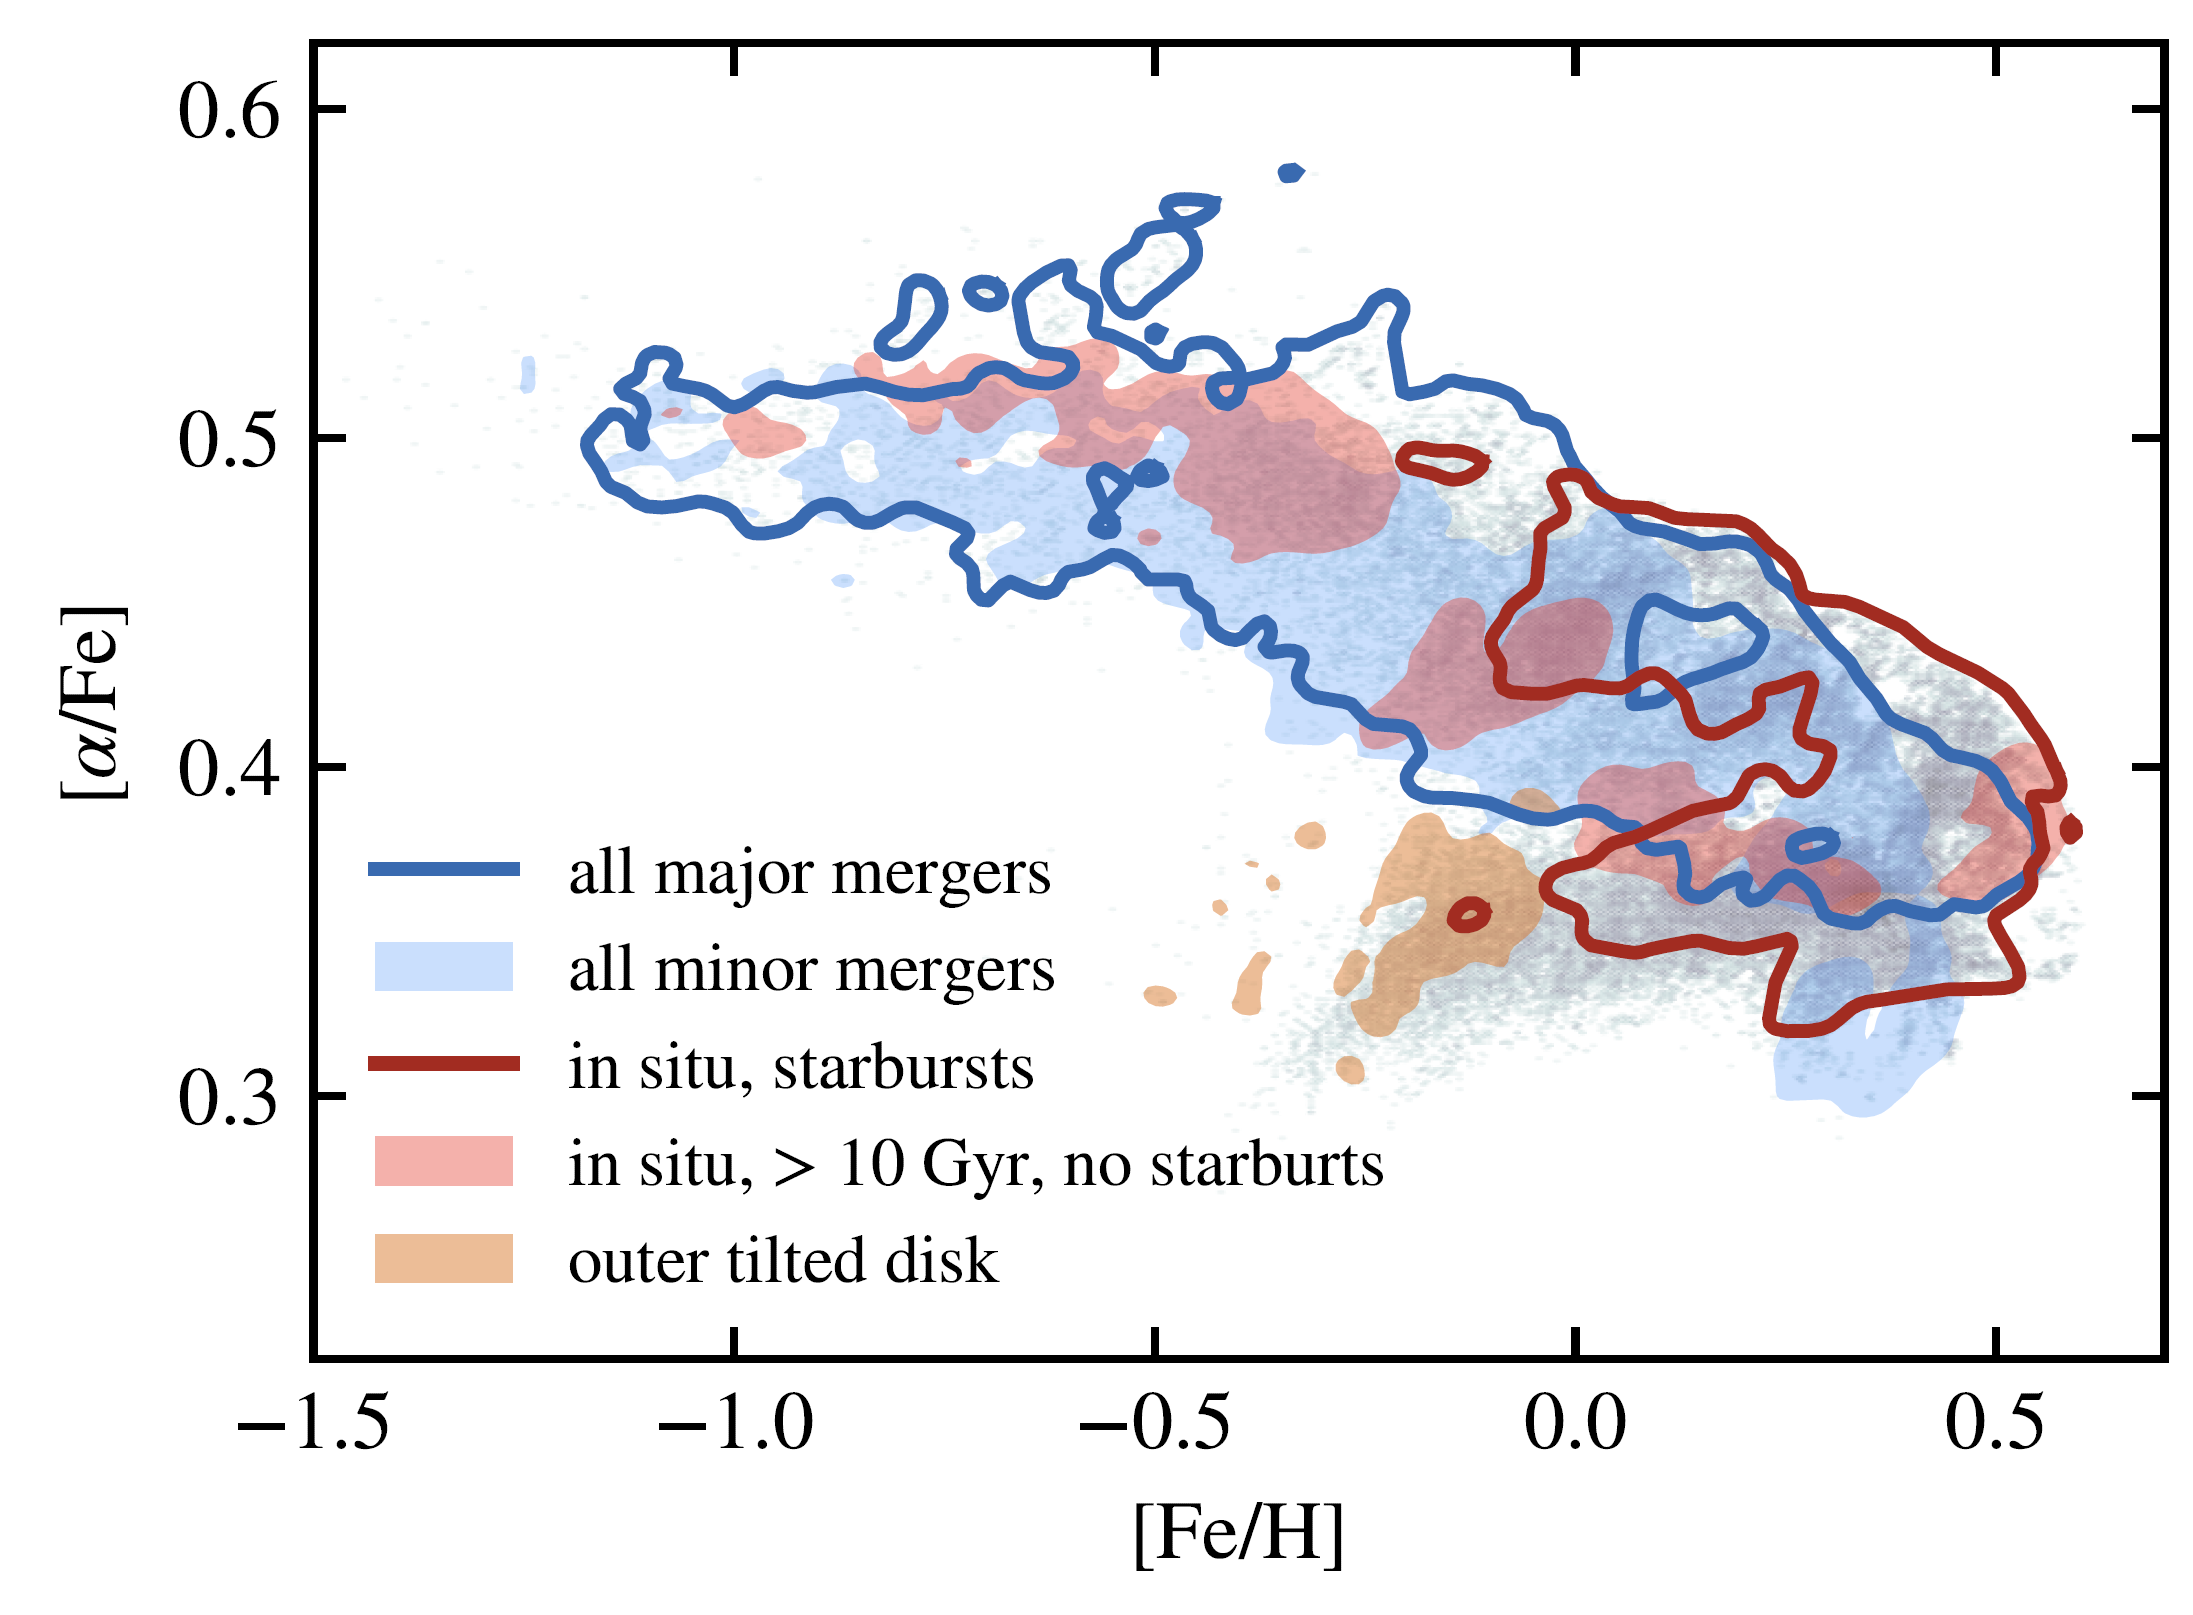
\includegraphics[width=0.8\textwidth]{images/vintergatan.png}
%    \vspace{-0.25cm}
%    \caption{Alpha-elements to iron abundances vs.\ metallicity, see text for explanation of notation. The grey dots in the background shows the chemical composition of stars found in the simulations with the coloured contours and regions mapping out the origin of their formation. Adapted from \citet{vintergatan:ii} with permission.} % Fig. 10
%    \label{fig:vintergatan}
%\end{figure}
%\begin{figure}[p]
%    \centering
%    \vspace{-0.5cm}
%    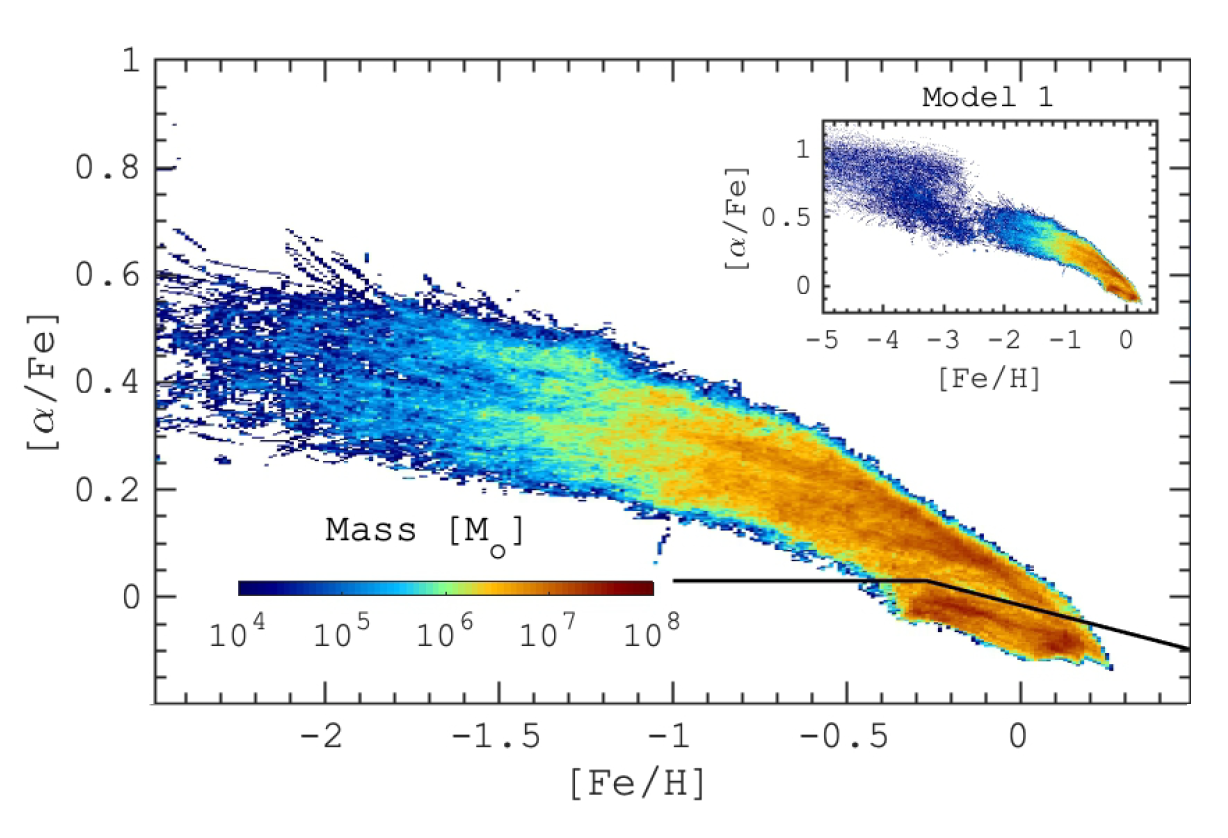
\includegraphics[width=0.8\textwidth]{images/khoperskovalpha.png}
%    \vspace{-0.25cm}
%    \caption{Alpha-elements to iron abundances vs.\ metallicity, colour-coded by the stellar mass, see text for explanation of notation. The frame in the top right is an overview of all the data in the simulation with the main figure itself a zoom-in. The black line separates two major stellar populations with low and high alpha-abundances. Adapted from \citet{khoperskov:20} with permission.} % Fig. 7
%    \label{fig:khoperskovalpha}
%\end{figure}
%\begin{figure}[p]
%    \centering
%    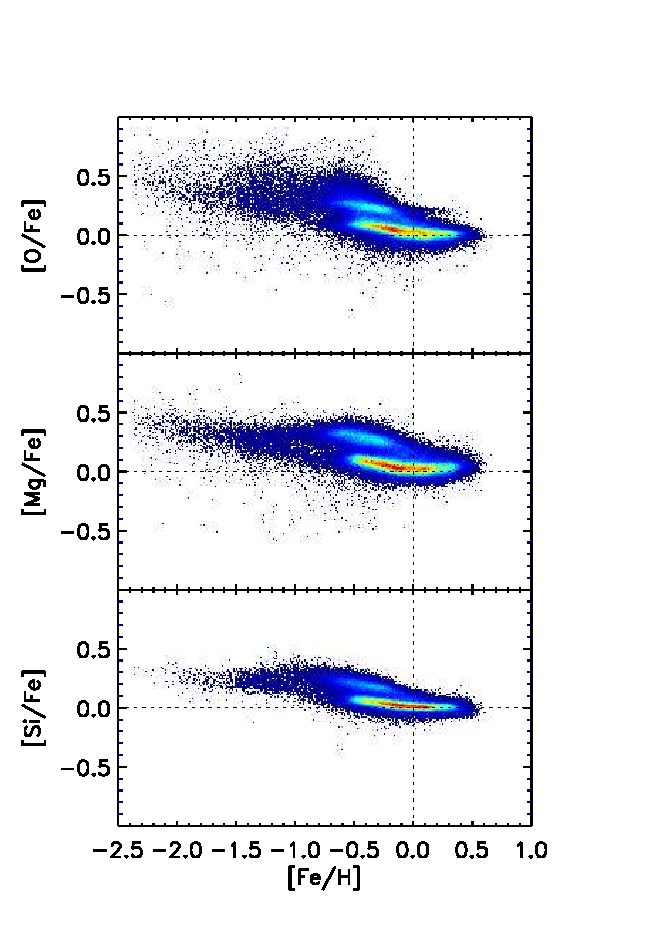
\includegraphics[trim={-0.3cm 0.9cm 0.8cm 1.8cm},clip,width=1.0\textwidth]{images/APOGEE_DR16_O_Mg_Si.pdf} % l b r t
%    \caption{Alpha-elements to iron abundances vs.\ metallicity, colour-coded by the stellar number density, see text for explanation of notation. The stars were observed as part of the APOGEE survey \citep{jonsson:20}, and shown here are the trends from giant stars for the three alpha-elements, O, Mg and Si. Figure from H.\ Jönsson (private communication).}
%    \label{fig:dr16}
%\end{figure}
%
%The notation [O/Fe] is to be understood as the abundance ratio of O to Fe logarithmically compared to the same ratio found in the Sun, as described by
%\begin{equation}
%    [\textrm{O}/\textrm{Fe}] = \log\left(\frac{N_\textrm{O}}{N_\textrm{Fe}}\right)_\textrm{star} - \log\left(\frac{N_\textrm{O}}{N_\textrm{Fe}}\right)_\textrm{Sun},
%\end{equation}
%where $N_\textrm{O}$ and $N_\textrm{Fe}$ are the number densities of O and Fe atoms respectively. The Sun is therefore located at the origin in the abundance plots. In Figure~\ref{fig:vintergatan} [\textalpha/Fe] is traced by [O/Fe] in the simulation, while in Figure~\ref{fig:khoperskovalpha} [\textalpha/Fe] is traced by the average of [O/Fe], [Mg/Fe] and [Si/Fe].
%
%Comparing the trends in Figures~\ref{fig:vintergatan} and \ref{fig:khoperskovalpha} to the trends in Figure~\ref{fig:dr16} shows the same high ratios that recede as the metallicity increases. In particular, the simulation can offer explanations for how the bimodal nature of the abundance trends arises from an evolution of the star formation activity in the galactic host. This is driven both by the transition from a merger-dominated growth phase in the early Universe to a quiescent evolution later, and the joint intrinsic evolution of the disks. Such matters are out of the scope of this thesis \citep[for details, see][]{vintergatan:ii}.
%
%\begin{figure}[t]
%    \centering
%    \vspace{-0.5cm}
%    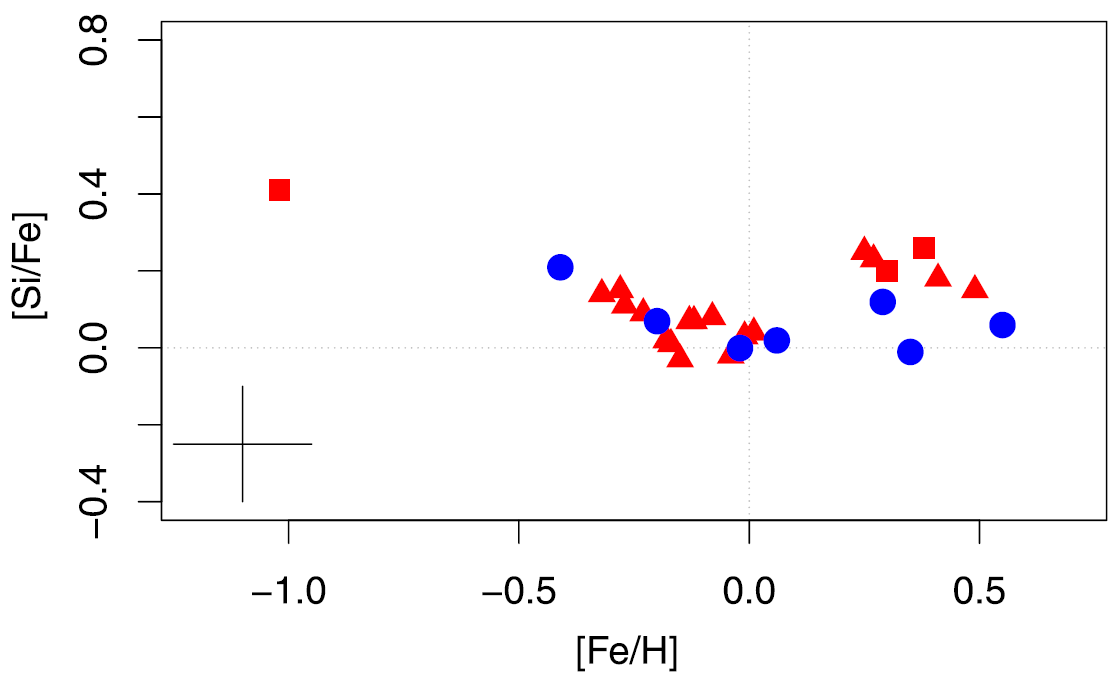
\includegraphics[width=0.8\textwidth]{images/thorsbroalpha.png}
%    \vspace{-0.25cm}
%    \caption{Alpha-elements to iron abundances vs.\ metallicity, here traced by Si, see text for explanation of notation. Red triangles and squares are abundances of stars found in the nuclear star cluster and nuclear stellar disk of the Milky Way; blue circles are stars found in the Milky Way disk. Adapted from \citet{thorsbro:20} with permission.} % Fig. 5
%    \label{fig:thorsbroalpha}
%\end{figure}
%
%The work in this thesis aims at adding observations of the Galactic centre to the available data. The data we have obtained is presented in the accompanying papers. One of our central results is shown here in Figure~\ref{fig:thorsbroalpha}. To our knowledge, there are currently no numerical simulations that have attempted to simulate the formation and evolution of the Galactic centre with a sufficient resolution to make a comparison to our data. In our Paper V we compare the data with chemical evolution models to offer possible interpretations of our data. It is our hope that with the availability of data like ours more theoretical work can be done to better understand the Galactic centre.



\section{Radial migration}\label{sect:radialmigration}

%In the previous section much attention is given to the diagnostic of alpha-elements and iron abundances. It is not a coincidence that this diagnostic of alpha-elements and iron abundances is both targeted by observers and included in the theoretical models. We take a closer look on first nucleosynthesis and then chemical evolution models to better understand why this diagnostic is interesting.
%
%\subsection{Nucleosynthesis}
%
%As mentioned in the previous section, the primordial gas initially present in the Universe shortly after the Big Bang mostly consists of hydrogen and helium (with a whiff of lithium and beryllium). All chemical species found today that are heavier than helium are therefore due to some fusion of the material originally found in the primordial gas. This is basically the domain of the stars. In astronomy all chemical species heavier than helium are called metals, and the metallicity of a gas is the amount of metal compared to hydrogen. Often the metallicity is traced by using the ratio of the abundance of iron atoms to hydrogen atoms (as we saw in the previous section with [Fe/H]), which has the underlying assumption that the distribution of metals in the given material is scaled to the distribution of metals we find in the Sun \citep[see e.g.][]{solar:sme}.
%
%Explaining how stars can form metals through various fusion processes is the domain of nucleosynthesis models, which is a vast scientific topic in itself \citep[see e.g.][]{burbidge:1957,woosley:95,kobayashi:20}. Here we focus on two production channels that are central for choosing the diagnostics discussed in the previous section. In these production channels metals are created through fusion and later released into the interstellar medium by either a supernova type II (SNII) or a supernova type Ia (SNIa) event.
%
%An SNII event happens towards the end of the life of a massive star with eight or more solar masses \citep[see e.g.][]{prialnik:00}. In such a massive star there is a significant production of the alpha-elements, which are then released to the interstellar environment through the SNII event. An alpha-particle is the nucleus of a helium atom, consisting of four nucleons, two protons and two neutrons. The alpha-particle is relevant because it has a particularly high binding energy per nucleon compared to the nuclei of other atoms, i.e. it is very tightly bound. This makes it a favoured product in fusion processes and as a consequence the combination of multiple alpha-particles also becomes favoured fusion products. In an SNII we see a strong production of several such alpha-elements, in particular the elements: O, Ne, Mg, Si, S, Ar, Ca and Ti.
%
%In comparison an SNIa event happens in binary systems, where one star has first developed into a white dwarf, and where the other star is undergoing its final stages of life and is transferring mass to the white dwarf. If enough mass is transferred to the white dwarf it collapses and ignites an SNIa event \citep[see e.g.][]{prialnik:00}. In an SNIa there is also the generation of alpha-elements, but the circumstances are such that the fusion processes are mainly focused around the production of iron and elements close to iron with respect to the number of protons, the so-called iron-peak elements: Ti, V, Cr, Mn, Fe, Co and Ni. Hence, an SNIa is seen as outputting iron, albeit a bit ``delayed'' as the two stars both have to go through their evolutionary stages before the output is seen.
%
%Ti requires more neutrons than protons to be stable and is therefore not really a true alpha-element, but since it is often produced together with the alpha-elements in type II supernovae it is sometimes considered to be an alpha-element by astronomers. An interesting side-effect of the unstable Ti created in an SNII is that it beta-decays to Sc, perhaps rendering Sc a better SNII tracer than Ti \citep{clayton:03}. However, the nucleosynthesis production channels are still under debate to this day, so one has to be careful about making definite statements.
%
%\subsection{Chemical evolution}
%
%In chemical evolution theories the basic premise is that stars are formed from the gas found in the interstellar medium (ISM). Over time the stars produce metals and return them to the ISM, which then forms the foundation for future generations of stars. Therefore the metallicity, [Fe/H], in a way becomes a proxy for cosmic time. How fast the [Fe/H] increases is dependent on the star formation rate (SFR) \citep[see e.g.][]{matteucci:12}.
%
%When gas infalls and starts producing stars, the mass distribution of the newly born stars can be described by the so-called initial mass function (IMF). The first IMF developed was by \citet{salpeter1955}, though there have been several revisions of this work since \citep[see e.g.\ historical overview by][]{kroupa:19}. It is interesting to note that while these IMFs have a theoretical foundation they have been fine-tuned to fit observations of the Milky Way.
%
%Since massive stars over-produce alpha-elements compared to other elements the ratio of alpha-elements to iron depends on the fraction of high mass stars created. However, over time the enhanced iron production from SNIa systems kicks in, at which the point the ratio of alpha-elements to iron drops. This leads to the famous ``alpha-knee plot'' first identified by \citet{matteucci:90}. An updated version of the figure, with IMF and SFR illustrated, is shown in Figure~\ref{fig:alphaknee}.
%
%\begin{figure}[t!]
%    \centering
%    \includegraphics[trim={0.65cm 5.5cm 0.3cm -4.2cm},clip,width=0.8\textwidth]{images/mb90fig.eps} % l b r t
%    \caption{\citet{matteucci:90} predicted that the knee in the trend of [O/Fe] with [Fe/H] depends on the star formation rate (SFR): High SFR systems, such as bulges and elliptical galaxies, should show enhanced [O/Fe] to high [Fe/H], whilst the low SFR dwarf galaxies show reduced [O/Fe] relative to the Solar vicinity. Also shown is the direction of the [O/Fe] plateau with an enhanced fraction of massive stars, marked as the initial mass function (IMF), which over-produce oxygen. Adapted from \citet{mcwilliam:16} with permission.} % Fig. 1
%    \label{fig:alphaknee}
%\end{figure}
%
%Figure~\ref{fig:alphaknee} demonstrates how the ratio of alpha-elements to iron vs.\ metallicity can be a diagnostic that provides a lot of information on the formation and evolutionary process that a stellar population has experienced.
%
%So far the evolution scenarios have been rather restricted to the simple infall of a gas cloud. Several advanced scenarios can be considered. For instance if a second gas cloud is accreted into the system, what happens then? Or what if there is a pause in the star formation process due to some event that suppresses star formation? These are some of the questions we explore in our work, which is explored in more detail in the accompanying papers.
%
%Or course, before such considerations can be taken into account, the actual observational data has to be gathered, which is the topic of the next section.


\section{Velocity distributions}\label{sect:velocitydistributions}

%It is hard to imagine the discipline of astronomy progressing without the science and engineering of instrumentation making high precision observations a reality. We have described in the earlier sections how observations are essential to constrain our theories. In this section the observations performed as part of the work done in this thesis are covered in some detail.
%
%The data analysed in this thesis has been obtained using the Keck II telescope during three observation visits at the W.\ M.\ Keck Observatory located on the volcano Mauna Kea on the island of Hawai'i (aka The Big Island), in the state of Hawaii in the U.S.A. We recognise and acknowledge the very significant cultural role and reverence that the summit of Mauna Kea has always had within the indigenous Hawaiian community. We have been most fortunate to have had the opportunity to conduct observations from this mountain.
%
%The Keck II telescope has a primary mirror of $\sim 10$\,m in diameter and comprises 36 hexagon segments that work together as a single unit. A photograph of the primary mirror taken during the first observational visit is shown in Figure~\ref{fig:keckii}. The telescope is constructed such that different instruments can be mounted to analyse the light that the telescope is capturing. For our work we have used the NIRSPEC spectrometer \citep{mclean:98}.
%
%\begin{figure}[p]
%    \centering
%    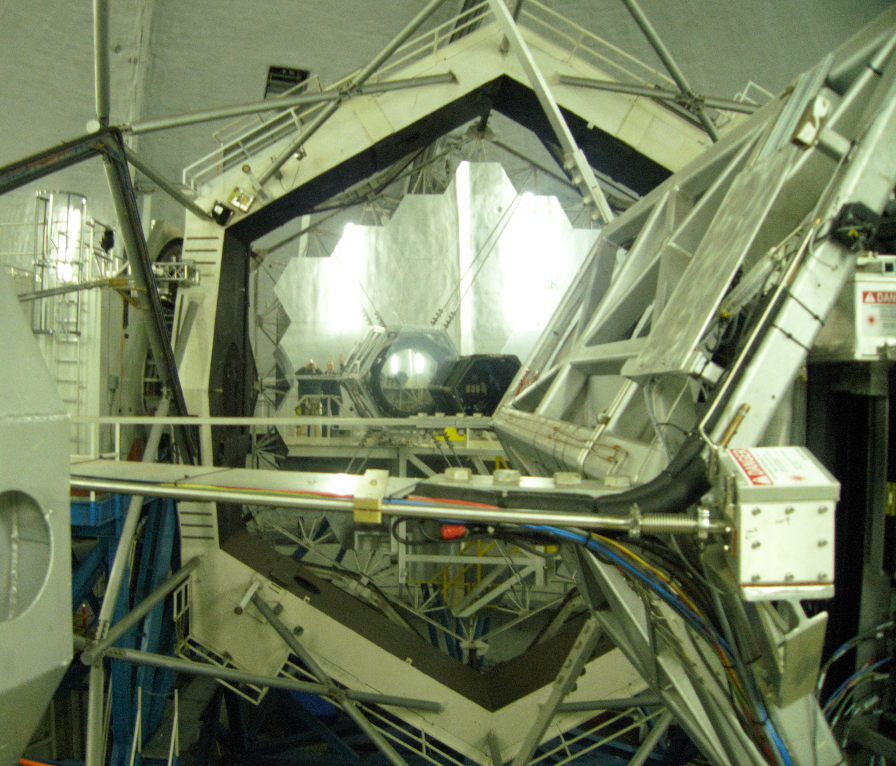
\includegraphics[width=1.0\textwidth]{images/keckii.png}
%    \caption{A photograph of the primary mirror of the Keck II telescope. The mirror is about 10\,m in diameter, illustrated by the size of the two people seen in the reflection (from the left Brian Thorsbro and Nils Ryde). The secondary mirror, which resides inside the metal box on the front right of the photograph, can be seen reflected in the primary mirror. The black hexagon, seen to the right of the reflection of the secondary mirror, is the focal point of the telescope where the captured light is gathered. From there the captured light is sent off to one of the mounted instruments. For our observations we used the NIRSPEC spectrometer that was mounted in one of the so-called Nasmyth/bent Cassegrain foci, located on the side of the telescope. Photograph by Brian Thorsbro.}
%    \label{fig:keckii}
%\end{figure}
%
%\begin{figure}[p]
%    \centering
%    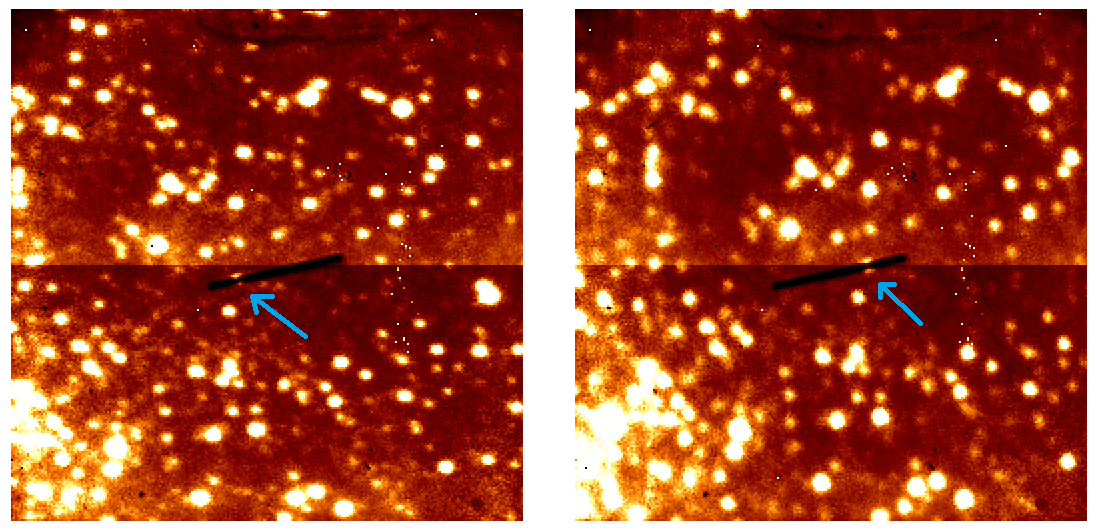
\includegraphics[width=1.0\textwidth]{images/gc13727scam.png}
%    \caption{Image taken with the Keck II telescope to verify that the target star, in this case the star named GC\,13727 in our work, is located correctly under the slit used to pass light on to the spectrometer. The blue arrows have been added to point out where the star is located. Two observations are performed using the ``nodding'' technique to ensure that it is also possible to obtain suitable background images for error subtraction.}
%    \label{fig:gc13727scam}
%\end{figure}
%\begin{figure}[p]
%    \centering
%    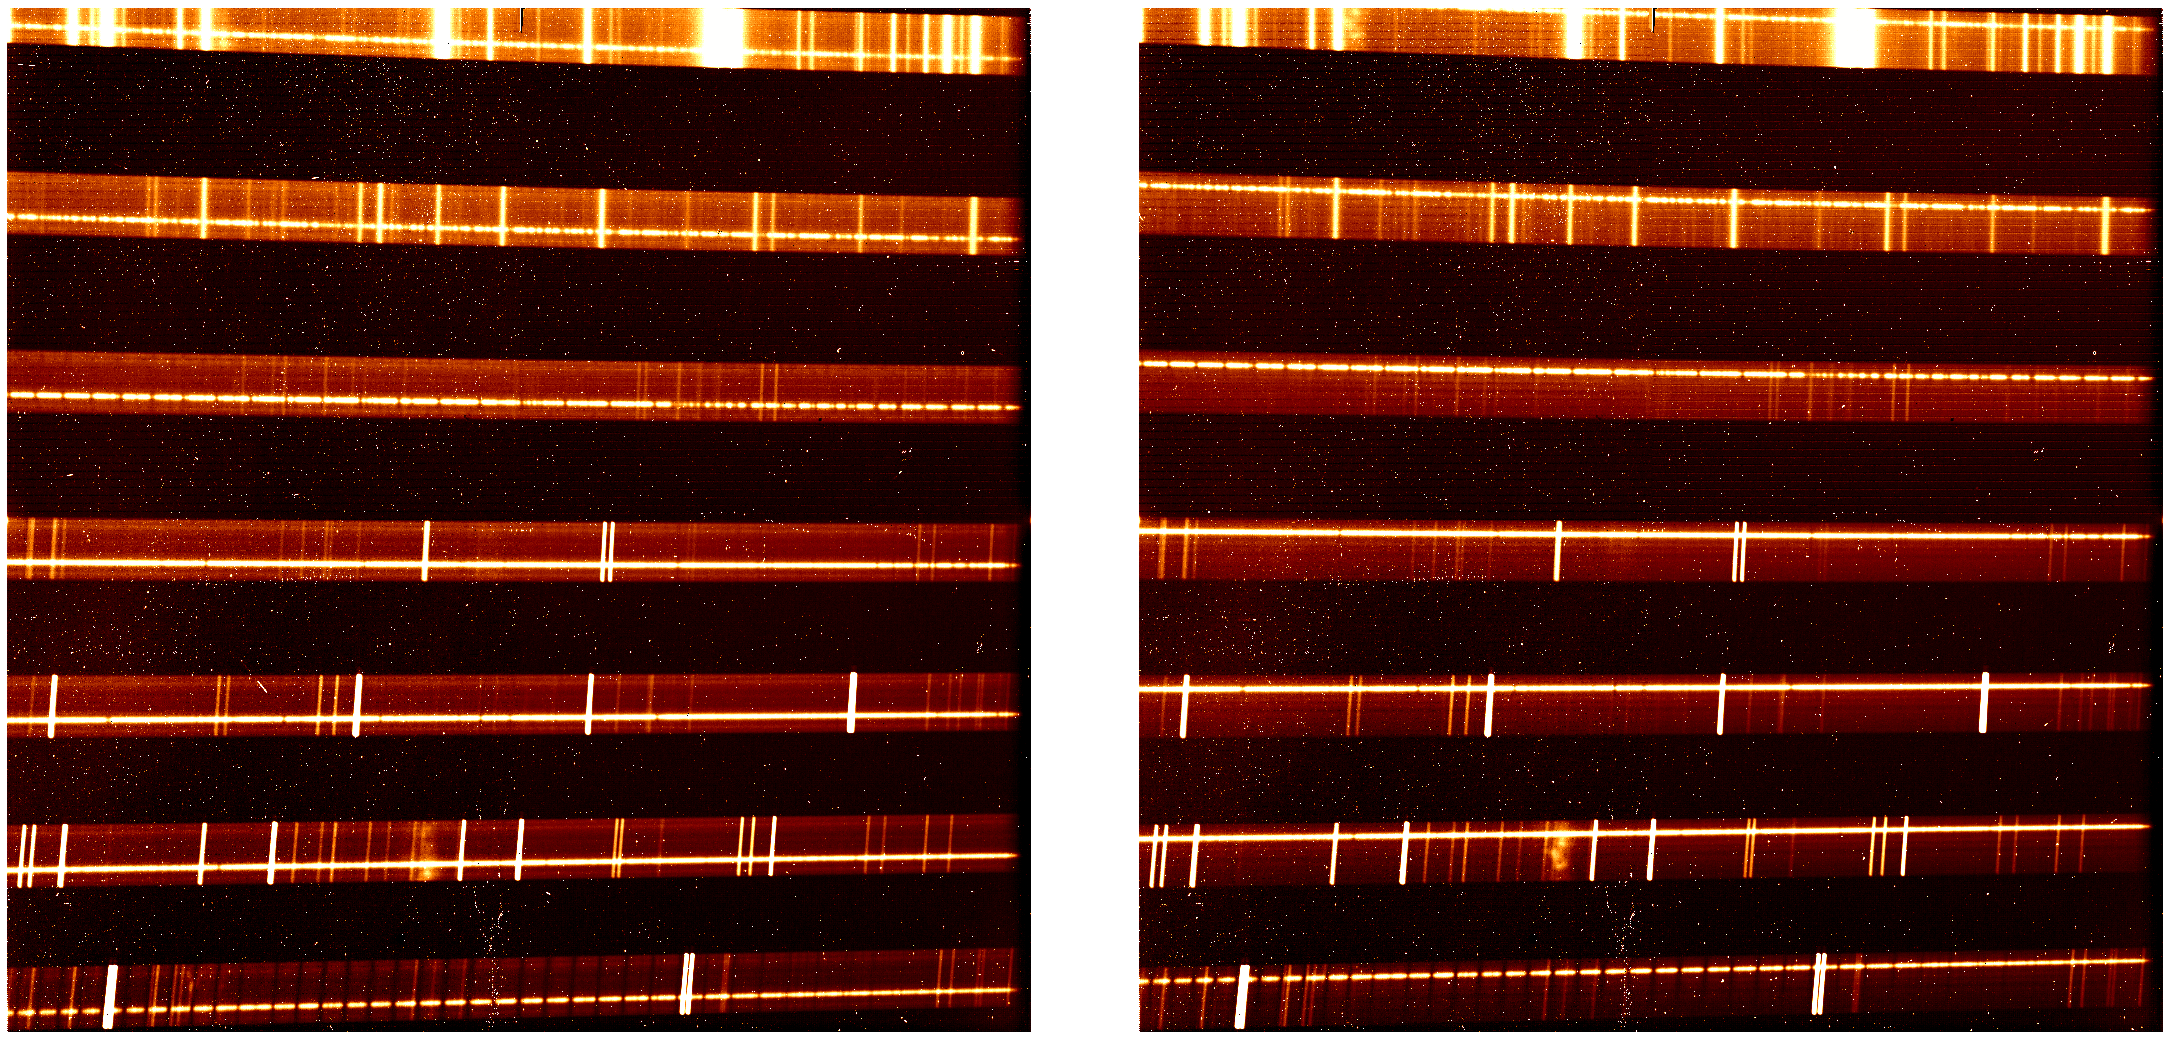
\includegraphics[width=1.0\textwidth]{images/gc13727speclight.png}
%    \caption{Observed cross-dispersed spectra of the same star, GC\,13727, as seen in Figure~\ref{fig:gc13727scam}. Absorption features can be seen as black ``Fraunhofer'' lines in various parts along the horizontal lines, which are the dispersed starlight. The vertical lines are OH emission lines from the Earth's atmosphere.}
%    \label{fig:gc13727spec}
%\end{figure}
%
%Observing the stars in the Galactic centre is particularly challenging because of the dust lying between the Sun and the Galactic centre. In the optical wavelength regime nearly all light is blocked. However, in the infrared wavelength regime around 2 micron about 15\% of the light penetrates through, which makes observations with large telescopes feasible. In our work we exposed the stars for about 40 minutes each on the Keck II telescope to reach a good signal to noise around 70 to 100. This is also the reason why we observe M giants, since they are very bright stars, with an apparent Ks magnitude around 11.
%
%The NIRSPEC spectrometer is a single slit spectrometer with a resolution of about R = 23,000. This is what we consider to be a necessary resolution for high quality abundance analyses. The slit of the spectrometer is placed on the star being observed, as illustrated in Figure~\ref{fig:gc13727scam}. We are interested in the light from the star, however the light passing through the rest of the slit can be used to quantify the background light. Subtracting background light allows for the reduction of systematic errors. This is especially important in the infrared, which is the wavelength region where we observe, since the thermal background is rather bright. Furthermore, there can be imperfections in the instrument that varies along the slit, so it is important to capture a background at the same slit location as the star, and to achieve this the telescope is ``nodded'', such that two observations are made. This way there will be two locations on the slit where the star is observed and for the same two slit positions there will also be a background observation. This ``nodding'' approach is shown in Figure~\ref{fig:gc13727scam} where blue arrows points to the location where the star is covered by the slit recording the light.
%
%The NIRSPEC spectrometer is a so-called cross-dispersed echelle spectrometer. This enables transverse dispersion of the recorded spectrum, such that a square detector array can be used more efficiently. In other words, the high resolution spectrum is cut up in parts and shifted vertically on the detector. An example of the image of a spectrum cut up in this way can be seen in Figure~\ref{fig:gc13727spec}. In this figure the horizontal lines are the spectrum of the observed star, and if one looks more closely it is possible to see black ``Fraunhofer'' lines, in particular in the third line from the top which displays molecular band absorption features of the molecule CO. The vertical lines are OH emission lines from Earth's atmosphere.
%
%In order to analyse the observed spectrum the spectral data has to be extracted from the image pixels. The Collaboration responsible for the design and implementation of the NIRSPEC spectrometer has made a software package available, called REDSPEC, which helps with this task \citep{nirspec_reduction}. The basic idea is to map out a curve that follows the spectrum across the pixels in the detector array and read out the intensity values along the curve. At the same time the software carries out background subtraction and divides out flat fields. The exact procedure will not be detailed here.
%
%Using the REDSPEC pipeline on the recorded image data we thus obtain a spectrum with an approximate wavelength calibration. Given that we observe in the infrared wavelength region around 2 microns we have many telluric features in the spectrum, which is both a blessing and a curse. It is helpful in improving the accuracy of the wavelength calibration, but it also means that parts of the spectrum are so crowded with telluric features that it can be difficult to reconstruct the actual stellar spectrum. Improving the wavelength calibration and removing the telluric features are performed by using the IRAF software package \citep{iraf}. For the telluric line removal we observe a swiftly rotating hot star which allows for easy identification of which spectral features that are telluric lines.
%
%However, in order to extract the abundances of chemical species, from the spectra that we observe we now turn to the field of stellar spectroscopy.


\section{Simulations}\label{sect:simulations}

%Spectroscopy was already founded in the 19th century when the dark Fraunhofer lines in the solar spectrum were identified to be the absorption of light caused by the presence of chemical species in the solar photosphere. The discovery was facilitated by shining light through different chemical species in a laboratory and recording at which wavelengths the light was absorbed. Up to the present day laboratory measurements are still a fundamental ingredient for the continued development of stellar spectroscopy \citep{nailingthestars2013}.
%
%Although the recording of the spectra of stars is important, an understanding is not reached until the underlying physics is well enough known to be able to reproduce the observed stellar spectra using physical modelling. The input needed for good modelling can broadly be categorised as
%\begin{itemize}
%    \item Atomic and molecular physics,
%    \item Stellar photospheres, and
%    \item Radiation transport.
%\end{itemize}
%
%A knowledge of these topics allows us to carry out abundance analyses of the observed stars. The topics are discussed in turn next, followed by a few pertinent comments on abundance analysis and astrophysical line lists.
%
%\subsection{Atomic and molecular physics}
%
%In modern atomic physics the state of an electron is described in a quantum mechanical way via a wave function. The energy level transition in an atom whereby an electron moves from one energy level to another is considered as a state change from one wave function to another. The electron has an electric charge and as the two wave functions have different probability distributions for the position of the electron there is a charge distribution difference between them, and thus there exists an electric dipole moment.
%
%This dipole interacts with the radiation field around the atom, and if the radiation field resonates with the natural frequency of the dipole then energy can be put into the atom in form of absorption or removed from the atom in form of stimulated emission. The natural frequency is also known as the wavelength of the transition. Knowing this to high precision is necessary to identify the lines in a spectrum.
%
%The dipole also has an oscillator strength, which can be hard to understand intuitively, but in a way it represents the probability that a transition will happen. The higher the chance for a transition the stronger the oscillator is said to be, and in the spectrum this manifests itself as a stronger line.
%
%In molecules there are similar energy transitions if the electrons in the atoms move around, but there are also energy transitions when switching between different rotational and vibrational modes of the molecule itself. The interactions of rotational and vibrational modes often gives rise to molecular bands, which consists of a large number of spectral lines grouped near each other in the spectrum.
%
%If one tries to identify all possible energy transitions that exist in our 92 naturally occurring elements, it amounts to a staggering number. On top of that the molecular data needs to be taken into account. In the infrared wavelength range, very few laboratory measurements have in fact been carried out, which makes stellar spectroscopy particularly challenging.
%
%One approach to obtaining usable atomic physics data is by employing theory to calculate the values. There are promising results showing that if theory is calibrated using measurements from the laboratory it can provide an avenue for cataloguing all this data \citep[e.g.][]{pehlivan:mg,pehlivan:sc17}.
%
%An important property of atoms with an odd number of nucleons, in particular if the number of protons is odd, is nuclear spin, which gives rise to hyperfine structure. If the nucleus of an atom has a nuclear spin the electronic energy levels in the atom are affected, and this has to be taken into account when calculating theoretical energy level transitions.
%
%\subsection{Stellar photospheres}
%
%The physical region in the star from where the radiation escapes is aptly named the photosphere and it is the region that determines the shape of the spectrum that we observe. Principally, the energy is generated in the interior of the star and is transported up to the photosphere through radiation transport and convection.
%
%The key parameters we are interested in are the temperature and pressure gradients of the photosphere, since they govern which chemical species can be detected. For simplicity, the photosphere is often only modelled in the radial direction, with so called 1D models, which provide a temperature and pressure stratification. Doing full 3D modelling would enable a higher fidelity on the heat transport from convection, which affects the temperature distribution. However, by employing mixing length theory this can be approximated to a good degree for stars like M giants, which has been shown by comparing 3D models with 1D models for giant stars \citep{cerni:17}.
%
%Performing a full 3D model would also enable us to understand the particle velocity fields in the photosphere, which is known to affect the spectra of the stars. However, for most stars we can not resolve the surface in any case, and the effect of the velocity fields can be approximated by introducing some heuristic parameters to the 1D modelling, usually denominated the micro- and macro-turbulence.
%
%Temperature is not an inherently unique property. In the same patch of space, the temperature described by the Maxwellian velocity distribution of particles is not necessarily the same temperature described by the Saha-Boltzmann equation, which is governed by the distribution of electrons in energy levels of chemical species. However, when the particle density is high, and collisions between particles dominate the energy distribution compared to the photon interactions from radiation fields, the system is said to be in local thermodynamic equilibrium (LTE). In LTE the radiation field becomes the Planck black body radiation field, and the temperature becomes unique.
%
%LTE is a very powerful assumption that enables physical modelling to be simplified tremendously. For stars like M giants most of the photosphere can be said to be in LTE. However, the outer parts of the photosphere can be sparse and cause the LTE condition to fall away. To a first order the non-LTE (or NLTE) condition can be modelled with perturbation theory, adding so-called departure coefficients to the Saha-Boltzmann equation.
%
%NLTE calculations for M giants have only been done to a limited extent. We did some calculations on Si for Paper V together with our collaborator Anish Amarsi showing the departure coefficients to be insignificant for our analysis. Other elements are now being calculated \citep[see e.g.][]{amarsi:20}, and will be published as they are completed.
%
%\subsection{Radiation transport}
%
%Radiation transport is quite simple in concept, namely that along a beam of light with a certain frequency, $\nu$, the change of intensity, $I$, of the radiation is governed by the intensity added and removed from the beam at a given position along the beam axis, $s$,
%\begin{equation}
%    \frac{\textrm{d}I(\nu,s)}{\textrm{d}s} = I_\textrm{added}(\nu,s) - I_\textrm{removed}(\nu,s).
%\end{equation}
%However, the intensities added and removed can originate from many different sources and sinks depending on the fidelity of the physical modelling.
%
%In LTE the intensity added to the light beam is described by the Planck black body radiation function. However, in NLTE the intensity added could depend on the radiation field, which in turn could depend on the intensity of the light beam, making a circular dependence that increases the difficulty of solving the radiation equation.
%%examples of radiation field dependence, photoionization and recombination
%
%The absorption of light at different frequencies varies, which leads to variations in how easy it is for the light to escape from the star as a function of frequency. If there are no chemical species to interact with the light of a given frequency the photon escaping the star could come from relatively deep regions of the star. If on the other hand the frequency of light matches a strong energy transition, most of the light at that frequency is absorbed, and only the photons from the very top of the star's surface are able to escape. The term opacity is used to describe how strongly light is being absorbed, and is a function of frequency.
%
%In cool stars the amount of free electrons and neutral hydrogen atoms are so plentiful that they interact with significant cross-sections in the following two absorption processes, which are respectively called $\textrm{H}^{-}$ bound-free and $\textrm{H}^{-}$ free-free \citep{1964MNRAS.128...93J}
%\begin{align}
%    \textrm{H}^{-} + \gamma &\longrightarrow \textrm{H} + \textrm{e}^{-} \\
%    \textrm{H} + \textrm{e}^{-} + \gamma &\longrightarrow \textrm{H} + \textrm{e}^{-}
%\end{align}
%\noindent In both cases the energy of the photon is transferred to the electron. The photon absorption by these two processes are both weak functions of the photon frequency and set a minimum opacity for the star. Such an opacity is often dubbed the continuum opacity. For stars like M giants, and incidentally also stars like the Sun, the continuum opacity in the optical and infrared wavelength ranges is dominated by the H$^{-}$ bound-free and free-free absorption processes \citep{1939ApJ....90..611W,1958ApJ...128..633C}. In general such a continuum opacity sets the limits on how deep we can probe into a star by observing escaped light.
%
%For transitions between energy levels in chemical species, and even for a change of rotational and vibrational modes for molecules, we call the process bound-bound absorption. In the frequency range where strong energy transitions exist the opacity becomes very high, which causes a strong spectral line to be present in the spectrum. The assumption that we can make is that the continuum and weaker spectral lines are created deeper in the photosphere, while the stronger absorption lines, in particular the core of these lines, are created further out in the photosphere.
%
%This means that for the continuum and the weaker lines we can normally assume that the LTE conditions hold, but for the stronger lines we need to be concerned whether NLTE conditions need to be taken into account, and if so, to what degree.
%
%\subsection{Abundance analysis}
%
%The spectral lines of chemical species are affected not only by the oscillator strength of a given transition, but also by the abundance of said species. Knowing both the oscillator strength and the abundance allows a spectral line to be modelled. However, as mentioned earlier, when the line becomes strong other considerations enter into the modelling, not only NLTE issues, but also saturation issues.
%
%Restricting ourselves to weak lines, a knowledge of the atomic and molecular physics of the chemical species and their abundances suffices to model the spectral line. This emphasises the importance of having the correct atomic and molecular physics information since it directly affects the abundance determination.
%
%Excellent tools exist that combine atomic physics data and stellar photosphere models, and solve the radiation equation using a set of stellar parameters and abundances of chemical species. For the atomic physics data one can download the dataset organised by the VALD3 Collaboration \citep{vald3}, and for stellar photosphere models the excellent MARCS models are a good choice \citep{marcs:08}. A tool that has been utilised many times throughout the work presented in this thesis is the code called Spectroscopy Made Easy, SME \citep{sme,sme_code,sme_evolution}.
%
%\subsection{Astrophysical line list}
%
%A challenge with the data found in the VALD3 collaboration \citep{vald3} is that large parts of the data have been calculated theoretically and have yet to be verified by laboratory measurements. This is a particular problem in the infrared wavelength regime. The theoretical calculations are very good, but aim at being correct on a statistical level to support opacity calculations for creating stellar atmosphere models, like the MARCS models \citep{marcs:08}.
%
%For stellar spectroscopy it is, however, necessary to verify every data point for every single spectral line. Assuming the abundances in the Sun are well known, one can produce model spectra of the Sun and compare to observations. Any deviation in line strength between model and observation can then be attributed to imprecise theoretical calculations in the oscillator strengths.
%
%Adjusting the oscillator strength to make the model spectra fit the observation of the Sun thus produces a new data set of oscillator strengths. These oscillator strengths are called astrophysical oscillator strengths to signify their non-laboratory origin.
%
%Another challenge with the data found in VALD3 is that the wavelength of a spectral line has an uncertainty associated with it, this goes not only for the theoretical calculations, but also for the laboratory measurements. Making accurate theoretical energy calculations is extremely difficult and requires very good physical modelling and often increases the reach of the problem beyond what can feasibly be calculated even with the most powerful computers today \citep[see e.g.][]{fischer:16}. The wavelength measurements obtained from laboratory experiments are not always as precise as we would like for high resolution spectroscopy, in particular because we need not only to assign the spectral lines to a given species, but also to be able to fit models to observations for abundance analysis.
%
%When comparing model spectra of the Sun with observations it becomes clear that, as with oscillator strengths, adjustments to the wavelength of a spectral line can be needed to fit model to observation. By combining the astrophysical oscillator strengths and the wavelength adjustments, an astrophysical line list is created.
%
%A major part of our work in this project has been to develop an astrophysical line list in the infrared wavelength regime around 2 microns. In total we identified more than 700 interesting spectral lines for our project and slightly modified about 570 of them \citep{thorsbro:17}.




\section{Outlook}\label{sect:outlook}

%The nuclear star cluster of the Milky Way is still poorly investigated with high resolution spectro\-scopy, which is needed for an accurate and precise abundance determination. Expanding our stellar sample to 100 stars or more would allow us to determine metallicities and abundances to a much higher degree, allowing us to confirm or reject the result suggested in Paper V. If the nuclear star cluster indeed is different from other stellar populations found elsewhere in the Galaxy, it is important to collect a good high resolution sample to map out the differences.
%
%It is possible to increase the resolution beyond the 23000 we have used, since for example NICRSPEC on the Keck telescopes has recently been upgraded to 38000, and other spectrometers exist, like IGRINS with a resolution of about 56000. IGRINS is also able to capture the H band ($\sim$\,1.5\,micron) in addition to the K band ($\sim$\,2\,micron), opening up an abundance analysis of many more chemical speciecs, though the higher extinction in the H band is a problem with current telescopes. The higher resolution will allow for higher fidelity in line detection and blend analysis.
%
%We are also interested in the exploration of the nuclear stellar disk. It is about 100 times more massive than the nuclear star cluster, and could be a more important component to study than the nuclear star cluster. We are planning on embarking on such a project with our collaborator R. M. Rich.
%
%In our current collected data set we have a few stars still under investigation that we are curious about (Thorsbro et al., in prep.). These stars are different from the stars included in our published work in that they are most probably young stars found in the nuclear star cluster. Their presence opens up the possibility of mapping the more recent star formation. Compared to earlier studies of these stars it is possible that we can advance our understanding of these stars by having more accurate and precise metallicity and abundance determinations from high resolution spectroscopy.
%
%We have also noticed a particularly high light element abundance in the stars we have observed, most likely nitrogen (Thorsbro et al., in prep.). It will be interesting to study this in further detail and determine if there is an actual difference between stars in the Galactic centre and stars further out in this respect. If this turns out to be an additional difference it will be another interesting observation that needs to be explained by theories.
%
%Finally, with the new large telescopes, 30\,m or more in diameter, new observation targets becomes available to us. Apart from seeing things further away, like stars in the Andromeda galaxy, M31, they can also be used for observing shorter wavelength regimes in dust-extincted regions compared to what we are able to do today. Being able to observe the nuclear star cluster in the H band could open up the abundance analysis of elements that do not have spectral lines in the K band.
%
%The future is bright.


% ===============================================================
% ====================== References:  ===========================
% depending on your field there can be a need for different styles etc.
% this example uses a style defined by American Astronomical Society journals

% Bibliography renamed to references
\renewcommand{\bibname}{References}
\bibliographystyle{aasjournal.bst}
%\let\jnl@style=\rmfamily
%\def\ref@jnl#1{{\jnl@style#1}}%
\def\ref@jnl#1{{#1}}%
\newcommand\aj{\ref@jnl{AJ}}%        % Astronomical Journal
\newcommand\araa{\ref@jnl{ARA\&A}}%  % Annual Review of Astron and Astrophys
\newcommand\apj{\ref@jnl{ApJ}}%    % Astrophysical Journal
\newcommand\apjl{\ref@jnl{ApJL}}     % Astrophysical Journal, Letters
\newcommand\apjs{\ref@jnl{ApJS}}%    % Astrophysical Journal, Supplement
\newcommand\ao{\ref@jnl{ApOpt}}%   % Applied Optics
\newcommand\apss{\ref@jnl{Ap\&SS}}%  % Astrophysics and Space Science
\newcommand\aap{\ref@jnl{A\&A}}%     % Astronomy and Astrophysics
\newcommand\aapr{\ref@jnl{A\&A~Rv}}%  % Astronomy and Astrophysics Reviews
\newcommand\aaps{\ref@jnl{A\&AS}}%    % Astronomy and Astrophysics, Supplement
\newcommand\azh{\ref@jnl{AZh}}%       % Astronomicheskii Zhurnal
\newcommand\baas{\ref@jnl{BAAS}}%     % Bulletin of the AAS
\newcommand\icarus{\ref@jnl{Icarus}}% % Icarus
\newcommand\jaavso{\ref@jnl{JAAVSO}}  % The Journal of the American Association of Variable Star Observers
\newcommand\jrasc{\ref@jnl{JRASC}}%   % Journal of the RAS of Canada
\newcommand\memras{\ref@jnl{MmRAS}}%  % Memoirs of the RAS
\newcommand\mnras{\ref@jnl{MNRAS}}%   % Monthly Notices of the RAS
\newcommand\pra{\ref@jnl{PhRvA}}% % Physical Review A: General Physics
\newcommand\prb{\ref@jnl{PhRvB}}% % Physical Review B: Solid State
\newcommand\prc{\ref@jnl{PhRvC}}% % Physical Review C
\newcommand\prd{\ref@jnl{PhRvD}}% % Physical Review D
\newcommand\pre{\ref@jnl{PhRvE}}% % Physical Review E
\newcommand\prl{\ref@jnl{PhRvL}}% % Physical Review Letters
\newcommand\pasp{\ref@jnl{PASP}}%     % Publications of the ASP
\newcommand\pasj{\ref@jnl{PASJ}}%     % Publications of the ASJ
\newcommand\qjras{\ref@jnl{QJRAS}}%   % Quarterly Journal of the RAS
\newcommand\skytel{\ref@jnl{S\&T}}%   % Sky and Telescope
\newcommand\solphys{\ref@jnl{SoPh}}% % Solar Physics
\newcommand\sovast{\ref@jnl{Soviet~Ast.}}% % Soviet Astronomy
\newcommand\ssr{\ref@jnl{SSRv}}% % Space Science Reviews
\newcommand\zap{\ref@jnl{ZA}}%       % Zeitschrift fuer Astrophysik
\newcommand\nat{\ref@jnl{Nature}}%  % Nature
\newcommand\iaucirc{\ref@jnl{IAUC}}% % IAU Cirulars
\newcommand\aplett{\ref@jnl{Astrophys.~Lett.}}%  % Astrophysics Letters
\newcommand\apspr{\ref@jnl{Astrophys.~Space~Phys.~Res.}}% % Astrophysics Space Physics Research
\newcommand\bain{\ref@jnl{BAN}}% % Bulletin Astronomical Institute of the Netherlands
\newcommand\fcp{\ref@jnl{FCPh}}%   % Fundamental Cosmic Physics
\newcommand\gca{\ref@jnl{GeoCoA}}% % Geochimica Cosmochimica Acta
\newcommand\grl{\ref@jnl{Geophys.~Res.~Lett.}}%  % Geophysics Research Letters
\newcommand\jcp{\ref@jnl{JChPh}}%     % Journal of Chemical Physics
\newcommand\jgr{\ref@jnl{J.~Geophys.~Res.}}%     % Journal of Geophysics Research
\newcommand\jqsrt{\ref@jnl{JQSRT}}%   % Journal of Quantitiative Spectroscopy and Radiative Trasfer
\newcommand\memsai{\ref@jnl{MmSAI}}% % Mem. Societa Astronomica Italiana
\newcommand\nphysa{\ref@jnl{NuPhA}}%     % Nuclear Physics A
\newcommand\physrep{\ref@jnl{PhR}}%       % Physics Reports
\newcommand\physscr{\ref@jnl{PhyS}}%        % Physica Scripta
\newcommand\planss{\ref@jnl{Planet.~Space~Sci.}}%  % Planetary Space Science
\newcommand\procspie{\ref@jnl{Proc.~SPIE}}%      % Proceedings of the SPIE

\newcommand\actaa{\ref@jnl{AcA}}%  % Acta Astronomica
\newcommand\caa{\ref@jnl{ChA\&A}}%  % Chinese Astronomy and Astrophysics
\newcommand\cjaa{\ref@jnl{ChJA\&A}}%  % Chinese Journal of Astronomy and Astrophysics
\newcommand\jcap{\ref@jnl{JCAP}}%  % Journal of Cosmology and Astroparticle Physics
\newcommand\na{\ref@jnl{NewA}}%  % New Astronomy
\newcommand\nar{\ref@jnl{NewAR}}%  % New Astronomy Review
\newcommand\pasa{\ref@jnl{PASA}}%  % Publications of the Astron. Soc. of Australia
\newcommand\rmxaa{\ref@jnl{RMxAA}}%  % Revista Mexicana de Astronomia y Astrofisica

%% added feb 9, 2016
\newcommand\maps{\ref@jnl{M\&PS}}% Meteoritics and Planetary Science
\newcommand\aas{\ref@jnl{AAS Meeting Abstracts}}% American Astronomical Society Meeting Abstracts
\newcommand\dps{\ref@jnl{AAS/DPS Meeting Abstracts}}% American Astronomical Society/Division for Planetary Sciences Meeting Abstracts

{\footnotesize\bibliography{references}}  % Link to bibtex file %%%%%%%%%%%%%%%%%%%

% ==================================
% ==================================
% ==================================
%
% ARTICLES
%
% ==================================
% ==================================
% ==================================

\chapterhidenum{Scientific publications}

\sectionhidenum{Paper summaries and author contributions}

A summary of each paper is presented here, and my contributions clarified.

\subsection*{Paper I}

In this paper we have gone through the first part of our dataset taken from the first observation trip. In the dataset we found a metal poor star in the hotter end of M giants with an effective temperature of about 3800 K. This means that its spectrum was devoid of most of the molecular features that we find in the other stars in our dataset. Hence, the star's spectrum was easier to analyse.

Careful orbit analysis of the star suggests that the star is a member of either the nuclear star cluster (NSC) or the nuclear stellar disk (NSD). The orbit does not show signs of it being a stray star from the bulge that has been captured, though we cannot rule out that the star may originally have formed in a globular cluster that had fallen into the Galactic centre.

That the star is metal poor, [Fe/H] $\sim -1.0$, meaning that it could be similar to globular cluster stars. Other studies of the Galactic centre are finding 5--10\% low metalliticy stars \citep{Feldmeier-Krause2017,do:15}, so our one star out of the 20 in our sample agrees with that.

We find that [\textalpha/Fe] $\sim 0.4$, which is similar to what is found elsewhere in our Galaxy for stars with the same metallicity. The study of this one star does not give reason to claim any differences between the Galactic centre and other parts of the Galaxy.

\subsubsection*{My contribution to paper I}

I took part in the observations, having led some of the time. I was responsible for the data reduction. I developed the astrophysical line list used for the spectroscopy analysis and carried out the abundance analysis in close collaboration with Nils Ryde. I contributed to writing the article.


\subsection*{Paper II}

In this paper we present a metallicity distribution function (MDF) of stars found in the nucleus of our Galaxy, either NSC or NSD. The stars seem to show two peaks in the MDF, one centred around [Fe/H]~$\sim -0.25$ and one centred around [Fe/H]~$\sim 0.4$.

Because of patchy extinction towards the Galactic centre, it turned out to be really difficult to get proper photometric $\log g$ values for all of the stars in the dataset. Given that we have targeted old stars we we were able to make use of the fact that isochrone tracks for M giants are insensitive to age for ages above 5\,Gyr. This means we have a function linking the three stellar parameters: effective temperature, [Fe/H] and $\log g$. Performing an iterative metallicity determination including the constraints from this developed function made it possible to determine the metallicities of the stars.

This method was verified against a subsample of giant stars in the APOGEE data set having effective temperatures between 3500 K and 4500 K so as to be as comparable to the M giants in our sample as possible. We also did the analysis using the photometric $\log g$ determinations, even though we had problems with the patchy extinction. The photometric results are in good agreement with the isochrone $\log g$ for many of the stars but, as expected, exhibit larger deviations for some of the stars.

We investigated many of the strong spectral lines belonging to scandium, titanium, vanadium and calcium. However, we found many lines to be very temperature sensitive and further suspected NLTE to be an issue, so we did not trust our abundance analysis of these lines.

\subsubsection*{My contribution to paper II}

I took part in the observations, having led some of the time. I was responsible for the data reduction. I used the previously developed astrophysical line list and did the abundance analysis in close collaboration with Nils Ryde. I developed the isochrone method required for finding the metallicity distribution. I contributed to writing the article.


\subsection*{Paper III}

After our paper II had been published, a publication \citep{do:18} appeared claiming unusual scandium, vanadium and yttrium abundances in the Galactic centre. We thus decided that it was necessary to return to the strong spectral lines we had ignored in Paper II and reconsider our data.

Our dataset also includes observations of M giants further out in the Galaxy that we use as a control sample. This allowed us to make a differential studies, where a lot of the systemic uncertainties are eliminated.

Comparing our Galactic centre stars and stars further out in the Galaxy, we found that these strong lines are also present further out in the Galaxy. Therefore, the strong lines are likely to be intrinsic to the cool stars that we are probing and not due to the stellar population or environment where the stars live.

We took a closer look at scandium, since we had recently measured its atomic properties in the lab. Many of the atomic physics properties of scandium were at the time not included in the database VALD3, and including them actually could explain partially the strong spectral lines. In particular temperature sensitivity due to ionisation and the hyperfine splitting properties of scandium are both significant contributors. Further investigation of the temperature sensitive NLTE effects will be needed to enable determination of Sc abundance from these lines.

\subsubsection*{My contribution to paper III}

I took part in the observations, having led some of the time. I was responsible for the data reduction. I used the previously developed astrophysical line list and isochrone method and carried out the Sc abundance determinations. I modelled scandium with and without hyperfine structure. I led the paper writing.


\subsection*{Paper IV}

This paper is unusual in that it started as a conference proceeding but, for some reason, it was assigned no less than three referees. Thanks to the comments from the referees it took off from there to become a work that focused on making the astrophysical results from the previous articles available to the atomic physics community.

\subsubsection*{My contribution to paper IV}

I was wholely responsible for this paper.


\subsection*{Paper V}

Since the publication of Paper II we have concentrated on finding good alpha lines to investigate. There are several good silicon lines and, after doing a thorough investigation into identifying molecular features of cool stars, we were able to compile a good set of silicon lines that could be used for abundance analysis.

After we had demonstrated the temperature sensitivity of scandium lines in Paper III we used this to implement a temperature determination function, rather similar to the CO bandhead one we have used in Paper II. It turned out that the temperatures determined from the scandium lines were generally in good agreement with the temperature from the CO bandhead method, which has increased our confidence in the determined effective temperatures of the stars.

Using the updates on molecular blending and the slightly improved temperatures, we redid the MDF analysis. It is quite similar to the MDF we found in Paper II, although the new MDF shows even more strongly the bimodality in the MDF suggested in Paper II.

We also investigated the silicon abundance as a tracer element for alpha elements and we find, curiously enough, a slightly enhanced silicon abundance for the metal-rich end of our dataset. We investigated possible systematics to be confident with the results. NLTE calculations showed that NLTE corrections are not a significant concern for our choice of silicon lines.

We entered into a collaboration with the community working on chemical evolution models and, in this paper, offer two possible explanations for the enhanced silicon abundances in metal-rich stars.


\subsubsection*{My contribution to paper V}

I took part in the observations, having led some of the time. I was responsible for the data reduction. I developed a scandium temperature determination method to improve on our temperatures. I used the previously developed astrophysical line list and isochrone method and performed the updated metallicity distribution and the abundance analysis. I investigated line blending by modelling theoretical spectra to minimise the impact of CN blending. I led the paper writing, including the coordination of contributions from the new collaborators.



% ==================================
% INSERT PAPERS
% ==================================
% Comment-out the 'includepdf' to compile faster while you are writing.

% PAPER I
\paperpagemark{Radial migration and vertical action in \textit{N}-body simulations}
%\includepdf[pages=-,width=1.20\textwidth,pagecommand={\thispagestyle{plain}}]{papers/mikkola_2020_migration}

% PAPER II
\paperpagemark{Detailed Abundances for the Old Population near the Galactic Center. I. Metallicity Distribution of the Nuclear Star Cluster}
%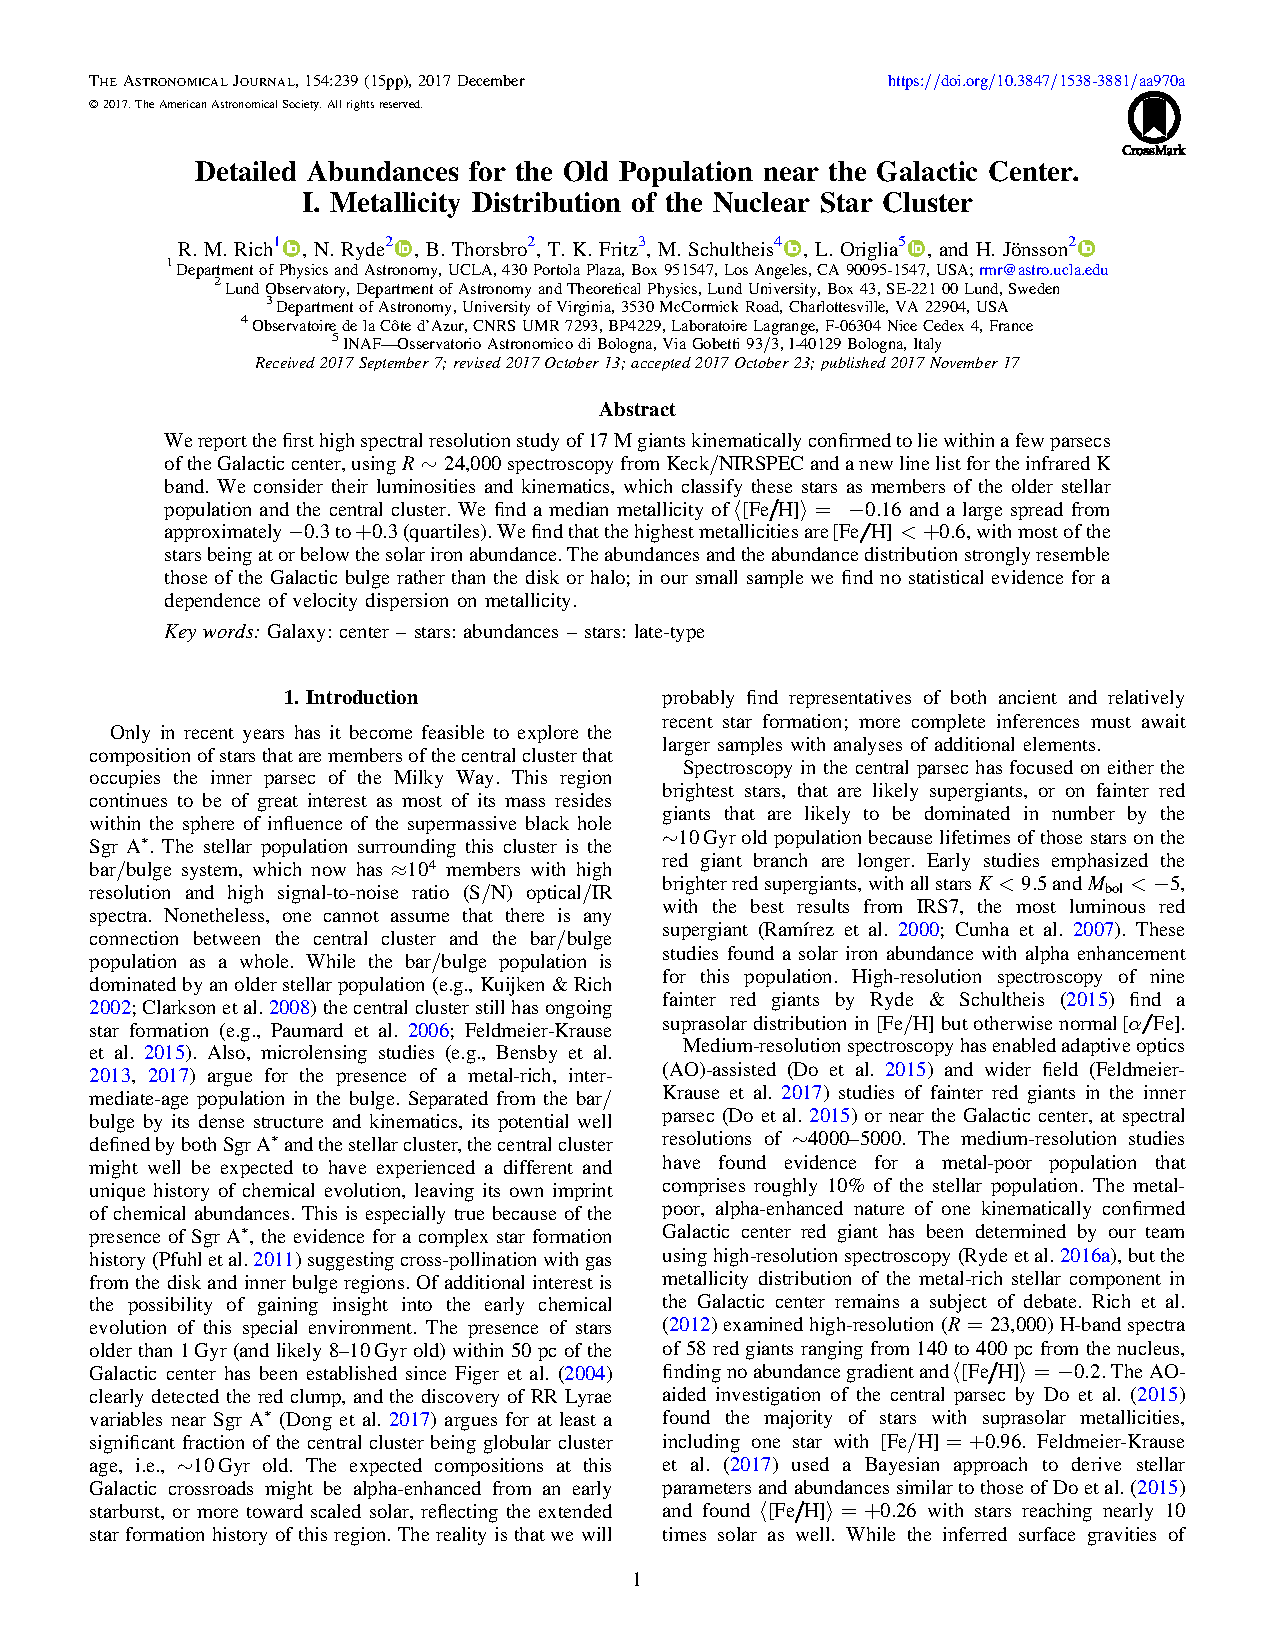
\includepdf[pages=-,width=1.20\textwidth,pagecommand={\thispagestyle{plain}}]{papers/rich_2017_mdf}

% PAPER III
\paperpagemark{Evidence against anomalous compositions for giants in the Galactic Nuclear Star Cluster}
%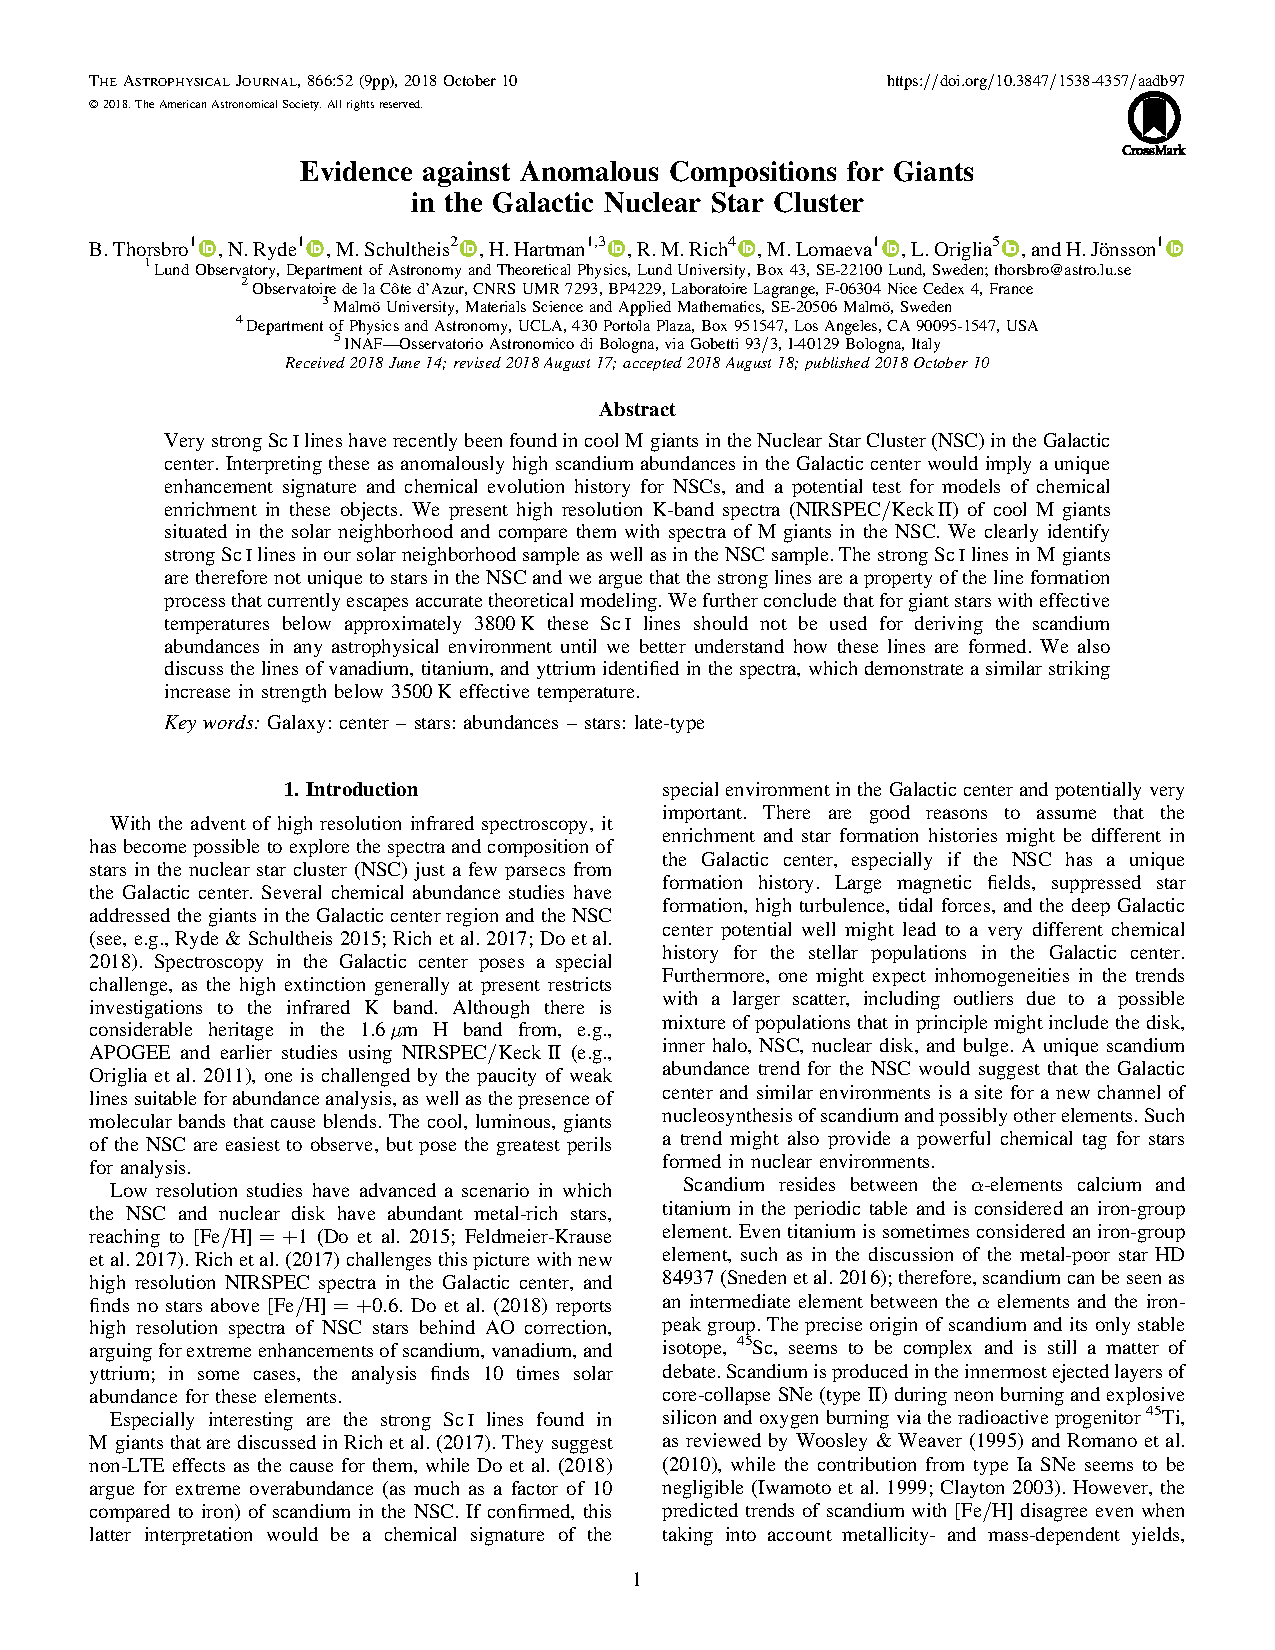
\includepdf[pages=-,width=1.20\textwidth,pagecommand={\thispagestyle{plain}}]{papers/thorsbro_2018_scandium}

% PAPER IV
\paperpagemark{Atomic Data Needs in Astrophysics: The Galactic Center ``Scandium Mystery''}
%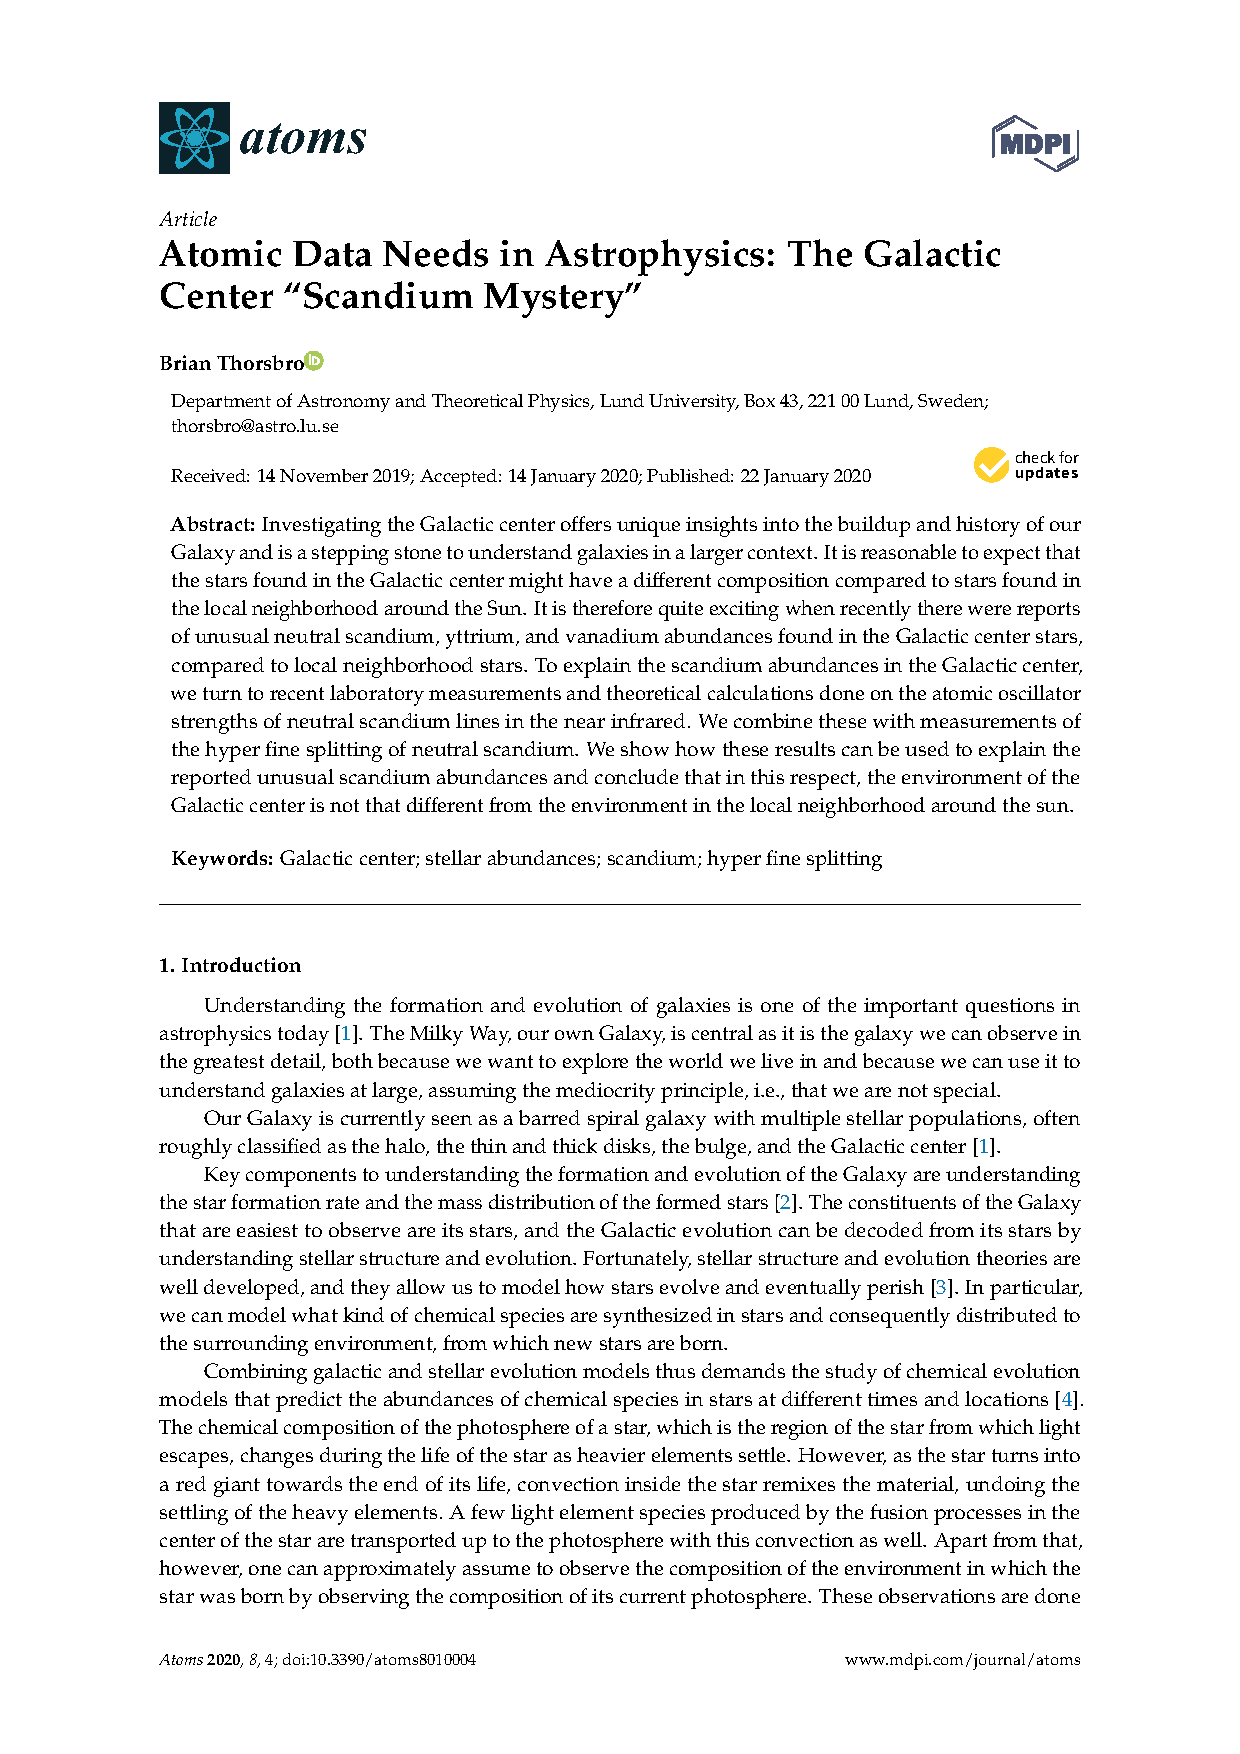
\includepdf[pages=-,width=1.20\textwidth,pagecommand={\thispagestyle{plain}}]{papers/thorsbro_2020_atoms}

% PAPER V
\paperpagemark{Detailed Abundances in the Galactic Center: Evidence of a Metal-rich Alpha-enhanced Stellar Population}
%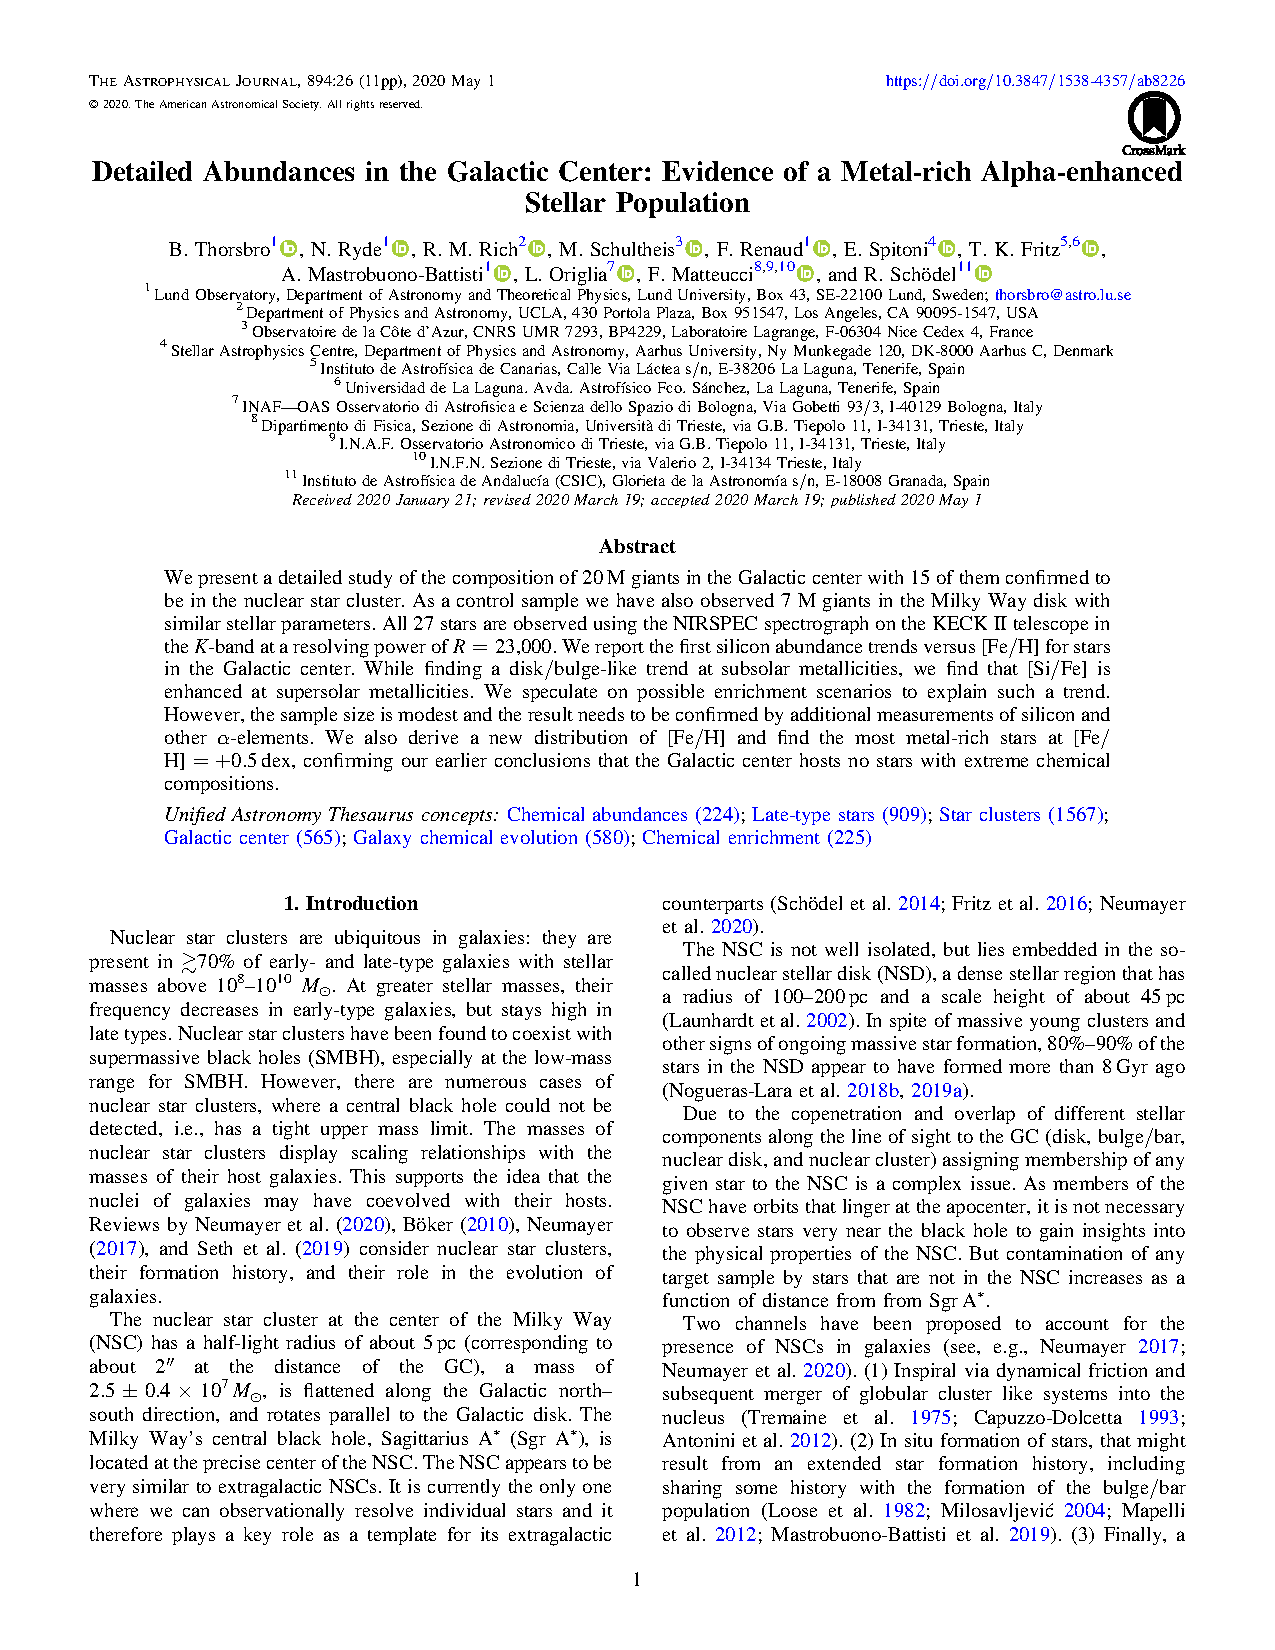
\includepdf[pages=-,width=1.20\textwidth,pagecommand={\thispagestyle{plain}}]{papers/thorsbro_2020_alpha}



\end{document}
